%\chapter{Elastic and Anelastic Perturbations}
\chapter{弹性和非弹性微扰}
\label{chap:spherperts}

在本章我们来确定微小的球对称扰动对~SNREI~或横向各向同性地球模型的简正模式本征频率的影响。利用瑞利原理,我们推导出球型或环型振荡本征频率的一阶微扰~$\delta\om$~用非微扰的径向本征函数表示的显式公式。通过考虑各向同性弹性参数的复数扰动,我们推导出由于体积非弹性的存在而导致的自由振荡品质因子倒数~$Q^{-1}$~的类似的一阶公式。这些结果为利用观测的地球自由振荡的本征频率和衰减率反演地球内部的球对称的平均弹性和非弹性结构提供了基础。

%\section{Spherical Perturbation}
\section{球对称微扰}
\index{perturbation!spherical|(}%

假设我们已知一个扰动前初始的球对称、无自转地球模型的本征频率~$\om$~和相应的径向本征函数~$U$,$V$,$P$~或~$W$,该地球模型的给定是由其密度~$\rho$~和相应重力加速度~$g$,以及各向同性模型的弹性参数~$\kappa$~和~$\mu$,或横向各向同性模型的~$C$,$A$,$L$,$N$~和~$F$。这些模型参数在几个内部的固-固或固-液界面以及外表面的半径~$d=a\cup d_{\rm SS}\cup d_{\rm FS}$~处会有不连续跃变。我们要来计算一个无穷小的球对称扰动的影响,该扰动由以下形式给定:
\begin{enumerate}
\item[(1)]
\index{perturbation!density}%
密度处处受到微扰,$\rho\rightarrow\rho+\delta\hspace{-0.2 mm}\rho$;
\item[(2)]
\index{perturbation!gravitational}%
重力加速度也处处受到微扰,$g\rightarrow g+\delta\hspace{-0.2 mm}g$;
\item[(3)]
\index{perturbation!elastic}%
弹性参数也受到微扰,$\kappa\rightarrow\kappa+\delta\kappa$,$\mu\rightarrow\mu+\delta\mu$~或~$C\rightarrow C+\delta C$,$A\rightarrow A+\delta A$,$L\rightarrow L+\delta L$,$N\rightarrow N+\delta N$,$F\rightarrow F+\delta F$;
\item[(4)]
\index{perturbation!in radius}%
最后,不连续面的半径有变动,$d\rightarrow d+\delta\hspace{-0.1 mm}d$,同时微扰后的密度、重力加速度和弹性参数都通过在微扰前的界面两侧做平滑外插而重新定义。
\end{enumerate}
重力加速度中的微扰与微扰~$\delta\hspace{-0.2 mm}\rho$~和~$\delta\hspace{-0.1 mm}d$~之间的关系为:
\eq  \label{eq:9.dg}
\delta\hspace{-0.2 mm}g(r)=4\pi Gr^{-2}\left\{
\int_0^r\delta\hspace{-0.2 mm}\rho'\,r^{\prime\hspace{0.2 mm}2}dr'
-\sum_{d<r}\delta\hspace{-0.1 mm}d\,d^2[\rho]^+_-\right\},
\en
其中第一项来自半径~$r$~以下的密度扰动,第二项来自所有半径~$d$~小于~$r$~的不连续面的移动。在下文中不必指定初始流体静力学压强~$p$~或其微扰~$\delta p$。
\index{perturbation!spherical|)}%

%\section{Application of Rayleigh's Principle}
\section{瑞利原理的应用}
\index{Rayleigh's principle!SNREI Earth|(}%
\label{section:perttheory}

由于地球模型中的这些变化,每个模式的本征频率都受到微扰:$\om\rightarrow\om+\delta\om$,相应的本征函数也受到微扰:$U\rightarrow U+\delta U$、$V\rightarrow V+\delta V$、$P\rightarrow P+\delta P$~或~$W\rightarrow W+\delta W$。瑞利原理使我们能够用扰动前的本征函数~$U$、$V$、$P$~或~$W$~来计算微扰~$\delta\om$,而无需同时求解微扰~$\delta U$、$\delta V$、$\delta P$~或~$\delta W$。为了统一处理球型、环型和径向振动,我们用通用的符号来表示相应的位移和位移-势函数作用量~$\sI_{\rm S}$、$\sI_{\rm T}$、$\sI_{\rm R}$~和~$\sI_{\rm S}^{\prime}$:
\eq \label{9.generI}
\sI=\int_0^{\infty}L(X,\dot{X};\om,\earth)\,r^2dr,
\en
\index{Euler-Lagrange equations!radial}%
其中~$X$~在球型拉格朗日量密度~(\ref{eq:8.spherl})~或~(\ref{eq:8.spherti})~中代表~$U$~和~$V$,在环型拉格朗日量密度~(\ref{eq:8.torl})~或~(\ref{eq:8.torti})~中代表~$W$,在径向拉格朗日量密度~(\ref{8.radI})~或~(\ref{8.RADTI})~中代表~$U$,而在修改后的球型拉格朗日量密度~(\ref{eq:8.spherl2})~或~(\ref{eq:8.sphertip})~中代表~$U$、$V$~和~$P$。考虑到最后一种情况,我们将~(\ref{9.generI})~中的积分上限写为~$\infty$,并在地球模型以外~$r>a$~的区域中定义~$U$、$V$~和~$W$~为零。拉格朗日量密度~$L$~中另外的参数表示其对本征频率~$\om$~和地球模型参数的依赖性;符号~$\earth$~在各向同性地球模型中包含~$\kappa$
、$\mu$、$\rho$~和~$g$,在横向各向同性地球模型中包含~$C$、$A$、$L$、$N$、$F$、$\rho$~和~$g$。瑞利原理的通用形式要求,对于任何可容许的变化~$\delta\hspace{-0.2 mm}X$,作用量~$\sI$~为稳定的条件是~$X$~满足欧拉-拉格朗日方程
\eq \label{9.ELeqn}
\p_XL-r^{-2}\frac{d}{dr}(r^2\p_{\dot{X}}L)=0,
\en
以及边界条件:$[\p_{\dot{X}}L]^+_-=0$,若~$X$~连续;$\p_{\dot{X}}L=0$,若~$X$~不连续。后一种情况是为了考虑在固-液边界~$r=d_{\rm FS}$~上切向滑移的可能性,并允许在自由表面~$r=a$~上的非零位移。

作用量的稳定值是~$\sI=0$,无论其取值是用不连续面在~$r=d$~的微扰前的地球模型~$\earth$~中的~$\om$~和~$X$,还是用不连续面在~$r=d+\delta\hspace{-0.1 mm}d$~的微扰后的地球模型~$\earth+\delta\earth$~中的~$\om+\delta\om$~和~$X+\delta\hspace{-0.2 mm}X$。精确到各种微扰的一阶,$\sI$~相对于包括~$\om$、$\earth$~和不连续面半径~$d$~在内的所有自变量的{\em 全变分\/}为
\index{total variation}%
\eqa \label{9.delItot}
\lefteqn{\delta\sI_{\rm total}=
\int_0^{\infty}[\delta\hspace{-0.2 mm}X(\p_XL)
+\delta\hspace{-0.2 mm}\dot{X}(\p_{\dot{X}}L)]\,r^2dr} \nonumber \\
&&\mbox{}+\int_0^{\infty}[\delta\om(\p_{\omega}L)
+\delta\earth(\p_{\subearth}L)]\,r^2dr
-\sum_d\delta\hspace{-0.1 mm}d\,d^2[L]^+_-=0,
\ena
其中对不连续面的求和是源自在混合区域因边界的移动而带来的积分的变化。同推导瑞利原理的做法一样,对包含有~$\delta\hspace{-0.2 mm}\dot{X}$~的项做分部积分,我们可以将方程~(\ref{9.delItot})~改写为
\eqa \label{9.delItot2}
\lefteqn{\delta\sI_{\rm total}=
\int_0^{\infty}\delta\hspace{-0.2 mm}X\!\left[\p_XL
-r^{-2}\frac{d}{dr}(r^2\p_{\dot{X}}L)\right]r^2dr} \nonumber \\
&&\mbox{}+\int_0^{\infty}[\delta\om(\p_{\omega}L)
+\delta\earth(\p_{\subearth}L)]\,r^2dr \nonumber \\
&&\mbox{}\qquad-\sum_dd^2[\delta\hspace{-0.2 mm}X(\p_{\dot{X}}L)+
\delta\hspace{-0.1 mm}d\,L]^+_-=0.
\ena

由欧拉-拉格朗日方程~(\ref{9.ELeqn}),(\ref{9.delItot2})~中的第一个积分为零。然而,此处的包含~$\delta\hspace{-0.2 mm}X$~的求和{\em 并不\/}为零,因为不连续面半径的扰动~$\delta\hspace{-0.1 mm}d$~使得变化~$\delta\hspace{-0.2 mm}X$~是{\em 不可容许的\/}。
\index{admissible variation}%
确保在扰动后边界两侧的微扰后本征函数~$X+\delta\hspace{-0.2 mm}X$~连续的一阶方程为~$[\delta\hspace{-0.2 mm}X]^+_-=
-\delta\hspace{-0.1 mm}d\,[\dot{X}]^+_-$。该条件对于~$r=d_{\rm FS}$~上的切向位移~$V$~和~$W$~不一定成立,对于~$r=a$~上的~$U$、$V$、$W$~也不一定成立;但是,$\p_{\dot{X}}L$~在这些情形下均为零,因此在所有边界~$r=d$~上,我们都必须有
\eq \label{9.Xcont}
[\delta X\hspace{0.3 mm}(\p_{\dot{X}}L)]^+_-=-\delta\hspace{-0.1 mm}d\,
[\dot{X}\hspace{0.3 mm}(\p_{\dot{X}}L)]^+_-
\en
将~(\ref{9.Xcont})~代入~(\ref{9.delItot2})~并重组各项,我们得到
\eqa
\label{9.PERT} \lefteqn{
\delta\om\int_0^{\infty}(\p_{\omega}L)\,r^2dr=-\int_0^{\infty}
\delta\earth(\p_{\subearth}L)\,r^2dr} \nonumber \\
&&\mbox{}+\sum_d\delta\hspace{-0.1 mm}
d\,d^2[L-\dot{X}(\p_{\dot{X}}L)]^+_-.
\ena
这是期望的结果,它使我们能够计算球对称、无自转地球模型由于其特性和不连续面半径的无穷小变化~$\delta\earth$~和~$\delta\hspace{-0.1 mm}d$~而引起的本征频率的一阶扰动~$\delta\om$。

在上面的推导中我们利用了径向作用量~(\ref{9.generI})~的两个性质:首先是瑞利原理,它要求在地球模型没有任何扰动的情况下,$\sI$~对任意可容许的变化~$\delta\hspace{-0.2 mm}X$~是稳定的;其次是能量均分关系,它确保总变分~$\delta\sI_{\rm total}$\hspace{0.2 mm}(即\hspace{0.2 mm}~$\sI$~在~$\om+\delta\om$、$X+\delta\hspace{-0.2 mm}X$、$\earth+\delta\earth$、$d+\delta\hspace{-0.1 mm}d$~和在~$\om$、$X$、$\earth$、$d$\hspace{0.2 mm}两者取值的差)为零。在没有任何边界扰动的情况下,用~$\delta\earth$~和扰动前本征函数~$X$~计算~$\delta\om$~的方法是经典的,已由~\textcite{rayleigh77}~给出来处理有限个自由度的系统。随后,\textcite{backus&gilbert67}~给出一个如~(\ref{9.PERT})~形式的公式,本来是能够处理~$\delta\hspace{-0.1 mm}d$~对地球自由振荡的影响的,但它忽略了~$-\dot{X}(\p_{\dot{X}}L)$~这一项。\textcite{woodhouse76}~首次得到了~(\ref{9.PERT})~式这一正确的结果,它考虑到本征函数微扰~$\delta\hspace{-0.2 mm}X$~的不可容许性。在第~9.3~节和第~9.4~节,我们会分别将方程~(\ref{9.PERT})~用于~SNREI~地球模型和横向各向同性地球模型。
\index{Rayleigh's principle!SNREI Earth|)}%

%\section{SNREI-to-SNREI Perturbation}
\section{SNREI~到~SNREI~微扰}
\index{perturbation!SNREI-to-SNREI|(}%
\label{section:isoper}

将控制~SNREI~地球的球型、环型和径向拉格朗日量密度~(\ref{eq:8.spherl})--(\ref{eq:8.torl})、(\ref{8.radI})~以及修改后的球型拉格朗日量密度~(\ref{eq:8.spherl2})~代入通用公式~(\ref{9.PERT})~式,我们得到
\eqa \label{9.ugly1}
\lefteqn{\delta\om\int_0^a(\p_{\omega}L_{\rm S})\,r^2dr} \nonumber \\
&&\mbox{}=-\int_0^a[\delta\hspace{-0.1 mm}
\kappa(\p_{\hspace{-0.3 mm}\kappa}L_{\rm S})
+\delta\hspace{-0.2 mm}\mu(\p_{\hspace{-0.3 mm}\mu}L_{\rm S})
+\delta\hspace{-0.2 mm}\rho(\p_{\hspace{-0.3 mm}\rho}L_{\rm S})
+\delta\hspace{-0.2 mm}g(\p_{\hspace{-0.3 mm}g}L_{\rm S})]\,r^2dr \nonumber \\
&&\mbox{}\qquad+\sum_d\delta\hspace{-0.1 mm}d\,d^2
[L_{\rm S}-\dU(\p_{\dot{U}}L_{\rm S})
-\dV(\p_{\dot{V}}L_{\rm S})]_-^+,
\ena
\eqa \label{9.uglyT}
\lefteqn{\delta\om\int_0^a(\p_{\omega}L_{\rm T})\,r^2dr=
-\int_0^a[\delta\hspace{-0.2 mm}\mu(\p_{\hspace{-0.3 mm}\mu}L_{\rm T})
+\delta\hspace{-0.2 mm}\rho
(\p_{\hspace{-0.3 mm}\rho}L_{\rm T})]\,r^2dr} \nonumber \\
&&\mbox{}+\sum_d\hspace{-0.1 mm}\delta d\,d^2
[L_{\rm T}-\dW(\p_{\dot{W}}L_{\rm T})]_-^+,
\ena
\eqa \label{9.ugly3}
\lefteqn{\delta\om\int_0^a(\p_{\omega}L_{\rm R})\,r^2dr} \nonumber \\
&&\mbox{}=-\int_0^a[\delta\hspace{-0.1 mm}
\kappa(\p_{\hspace{-0.3 mm}\kappa}L_{\rm R})
+\delta\hspace{-0.2 mm}\mu(\p_{\hspace{-0.3 mm}\mu}L_{\rm R})
+\delta\hspace{-0.2 mm}\rho(\p_{\hspace{-0.3 mm}\rho}L_{\rm R})
+\delta\hspace{-0.2 mm}g(\p_{\hspace{-0.3 mm}g} L_{\rm R})]\,r^2dr \nonumber \\
&&\mbox{}\qquad+\sum_d\delta\hspace{-0.1 mm}d\,d^2
[L_{\rm R}-\dU(\p_{\dot{U}}L_{\rm R})]_-^+,
\ena
\eqa \label{9.ugly4}
\lefteqn{\delta\om\int_0^{\infty}(\p_{\omega}L_{\rm S}^{\prime})\,r^2dr} \\
&&\mbox{}=-\int_0^{\infty}[\delta\hspace{-0.1 mm}
\kappa(\p_{\hspace{-0.3 mm}\kappa}L_{\rm S}
^{\prime})+\delta\hspace{-0.2 mm}\mu
(\p_{\hspace{-0.3 mm}\mu}L_{\rm S}^{\prime})
+\delta\hspace{-0.2 mm}\rho(\p_{\hspace{-0.3 mm}\rho}L_{\rm S}^{\prime})
+\delta\hspace{-0.2 mm}g
(\p_{\hspace{-0.3 mm}g} L_{\rm S}^{\prime})]\,r^2dr \nonumber \\
&&\mbox{}\qquad+\sum_d\delta\hspace{-0.1 mm}d\,d^2
[L_{\rm S}^{\prime}-\dU(\p_{\dot{U}}L_{\rm S}
^{\prime})-\dV(\p_{\dot{V}}L_{\rm S}^{\prime})
-\dP(\p_{\dot{P}}L_{\rm S}^{\prime})]_-^+, \nonumber
\ena
其中我们在必要时将积分上限换成了地球半径~$a$。对于地幔环型模式,\ref{9.uglyT}~式中的积分上下限可以分别换成~$s$~和~$b$,而内核环型模式的上限可以用~$c$~替换;求和同样仅包含地幔和内核中的不连续面~$d$。用本书所采用的归一化~(\ref{8.sphort})--(\ref{8.totort}),(\ref{9.ugly1})--(\ref{9.ugly4})~的左边都简化为~$\om\,\delta\om$。在对其右边做所示的微分后,我们发现~SNREI~地球模型的球型、环型或径向自由振荡的本征频率的微扰可以用~$\delta\hspace{-0.1 mm}\kappa$,$\delta\hspace{-0.2 mm}\mu$,$\delta\hspace{-0.2 mm}\rho$~和~$\delta\hspace{-0.1 mm}d$~这四项扰动表示为:
\eq \label{eq:9.delomiso}
\delta\om=
\int_0^a(\delta\hspace{-0.1 mm}\kappa\hspace{0.3 mm}K_{\kappa}
+\delta\hspace{-0.2 mm}\mu\hspace{0.3 mm}K_{\mu}
+\delta\hspace{-0.2 mm}\rho\hspace{0.3 mm}K_{\rho})\,dr
+\sum_d\delta\hspace{-0.1 mm}d\,[K_d]_-^+,
\en
其中
\eq
2\om K_{\kappa}=(r\dU+2U-\sqL V)^2, \label{eq:9.Kkap}
\en
\eqa \label{eq:9.Kmu}
\lefteqn{2\om K_{\mu}=\third(2r\dU-2U+\sqL V)^2} \nonumber \\
&&\mbox{}+(r\dV-V+\sqL U)^2+(r\dW-W)^2 \nonumber \\
&&\mbox{}\qquad+(\sqL^2 -2)(V^2+W^2),
\ena
\eqa \label{eq:9.Krho}
\lefteqn{2\om K_{\rho}=-\om^2r^2(U^2+V^2+W^2)+8\pi G\rho r^2U^2} \nonumber \\
&&\mbox{}+2r^2(U\dP+\sqL r^{-1}VP)-2grU(2U-\sqL V) \nonumber \\
&&\mbox{}\qquad-8\pi Gr^2\int_r^a\rho^{\prime}
U'(2U'-\sqL V')\,r^{\prime -1} dr',
\ena
\eqa \label{eq:9.Kd}
\lefteqn{2\om K_d=-\kappa(2\om K_{\kappa})-\mu(2\om K_{\mu})
-\rho(2\om K_{\rho})} \nonumber \\
&&\mbox{}+2\kappa r\dU(r\dU+2U-\sqL V)
+\fourthirds\mu r\dU(2r\dU
-2U+\sqL V) \nonumber \\
&&\mbox{}\qquad+2\mu r\dV(r\dV-V+\sqL U)
+2\mu r\dW(r\dW-W).
\ena
为简洁起见,我们将所有三种模式的结果整合在~(\ref{eq:9.Kkap})--(\ref{eq:9.Kd})~中;对于球型模式,我们将~$W$~设置为零,对于环型模式,将~$U$、$V$、$P$~设置为零,对于径向模式,将~$V$~和~$W$~设置为零。利用了基于~(\ref{eq:9.dg})~的分部积分来消除对重力微扰~$\delta\hspace{-0.2 mm}g$~的依赖性:
\eqa
\lefteqn{\int_0^a\delta\hspace{-0.2 mm}g\,[2\rho r^{-1}
U(2U-\sqL V)]\,r^2 dr} \nonumber \\
&&\mbox{}=8\pi G\int_0^a\delta\hspace{-0.2 mm}\rho
\int_r^a\rho^{\prime}U'(2U'-\sqL V')\,r^{\prime -1}dr'\,r^2dr \nonumber \\
&&\mbox{}-8\pi G\sum_d\delta\hspace{-0.1 mm}d\,d^2\,[\rho]^+_-
\int_r^a\rho^{\prime}U'(2U'-\sqL V')\,r^{\prime -1}dr'.
\ena
如预期的,(\ref{9.ugly1})~和~(\ref{9.ugly4})~两式导致相同的结果;如同~(\ref{8.Pexplicit})~所表示的,在计算修改前的球型作用量的导数~$\p_{\hspace{-0.3 mm}\rho}L_{\rm S}$~时,有必要考虑~$P$~对密度的依赖性。所谓的~{\em Fr\'{e}chet
积分核\/}~$K_{\kappa}$,$K_{\mu}$,$K_{\rho}$~和~$K_d$~提供了简正模式对不可压缩性~$\delta\hspace{-0.1 mm}\kappa$、刚度~$\delta\hspace{-0.2 mm}\mu$、密度~$\delta\hspace{-0.2 mm}\rho$和不连续面半径~$\delta\hspace{-0.1 mm}d$~的球对称微扰的敏感性提供了直接的衡量方法。
\index{Fr\'{e}chet kernel}%
\index{kernel!Fr\'{e}chet}%

许多模式的本征频率主要取决于纵波速度~$\alpha$~或横波速度~$\beta$,而对密度~$\rho$~只有微弱的依赖性。为了明确地表示这种敏感性,可以利用以下一阶关系方便地将微扰~$\delta\om$~用~$\delta\hspace{-0.1 mm}\alpha$,$\delta\hspace{-0.2 mm}\beta$,$\delta\hspace{-0.2 mm}\rho$~而不是~$\delta\hspace{-0.1 mm}\kappa$,$\delta\hspace{-0.2 mm}\mu$,$\delta\hspace{-0.2 mm}\rho$~来表示
\eq \label{9.dkappa}
\delta\hspace{-0.1 mm}\kappa=\delta\hspace{-0.2 mm}\rho
(\alpha^2-\fourthirds\beta^2)+2\rho(\alpha\,\delta\hspace{-0.1 mm}\alpha
-\fourthirds\beta\,\delta\hspace{-0.2 mm}\beta),
\en
\eq \label{9.dmu}
\delta\hspace{-0.2 mm}\mu=\delta\hspace{-0.2 mm}\rho
\,\beta^2+2\rho\beta\,\delta\hspace{-0.2 mm}\beta.
\en
将~(\ref{9.dkappa})--(\ref{9.dmu})~代入~(\ref{eq:9.delomiso}),我们得到
\eq
\delta\om=
\int_0^a(\delta\hspace{-0.1 mm}\alpha\hspace{0.3 mm}K_{\alpha}
+\delta\hspace{-0.2 mm}\beta\hspace{0.3 mm}K_{\beta}
+\delta\hspace{-0.2 mm}\rho\hspace{0.3 mm}
K_{\raisebox{0.3 ex}{\scriptsize$\rho$}}^{\prime})\,dr
\label{eq:9.delomiso2}
+\sum_d\delta\hspace{-0.1 mm}d\,[K_d]_-^+,
\en
其中
\eq
K_{\alpha}=2\rho\alpha K_{\kappa}, \label{eq:9.Kalpha}
\en
\eq
K_{\beta}=2\rho\beta(K_{\mu}-\fourthirds K_{\kappa}), \label{eq:9.Kbeta}
\en
\eq
K_{\raisebox{0.3 ex}{\scriptsize$\rho$}}^{\prime}=
(\alpha^2-\fourthirds\beta^2)K_{\kappa}+\beta^2K_{\mu}
+K_{\rho}. \label{eq:9.Krhop}
\en
在对~SNREI~地球参考模型加以改进时,只要应用了体波走时数据和简正模式本征频率数据,使用~Fr\'{e}chet~积分核~$K_{\alpha}$、$K_{\beta}$、$K_{\raisebox{0.3 ex}{\scriptsize$\rho$}}^{\prime}$~和~$K_d$~的表达式~(\ref{eq:9.delomiso2})~显然比~(\ref{eq:9.delomiso})~式更合适。

笼统来讲,(\ref{eq:9.delomiso})~和~(\ref{eq:9.delomiso2})~两式使我们能够计算~$\omega$~相对于地球模型的依赖深度性质的一阶{\em 偏导数\/}。
\index{partial derivative}%
例如,我们可以写出:
\eq \label{9.pderiv}
\left(\frac{\p\om}{\p\alpha}\right)_{\beta,\rho,d}
=K_{\alpha},\qquad\,
\left(\frac{\p\om}{\p\beta}\right)_{\alpha,\rho,d}
=K_{\beta}, \nonumber
\en
\eq \label{9.pderiv2}
\left(\frac{\p\om}{\p\hspace{-0.2 mm}\rho}\right)_{\alpha,\beta,d}
=K_{\raisebox{0.3 ex}{\scriptsize$\rho$}}^{\prime},\qquad
\left(\frac{\p\om}{\p d}\right)_{\alpha,\beta,\rho}
=K_d,
\en
其中下角标指明了在微分过程中保持固定的变量。相对于不可压缩性、刚度和密度的偏导数的定义与原来的~Fr\'{e}chet~积分核~$K_{\kappa}$,$K_{\mu}$~和~$K_{\rho}$~类似。

利用动能-势能均分关系~$\om^2\sT=\sV_{\kappa}+\sV_{\mu}+\sV_{\rm g}$,我们发现当保持地震波速~$\alpha$~和~$\beta$~固定时,对密度~$\rho$~的偏导数满足
\eqa \label{9.Guust} \lefteqn{2\om
\int_0^a\rho\left(\frac{\p\om}
{\p\hspace{-0.2 mm}\rho}\right)_{\alpha,\beta,d}\,dr
=\int_0^a[4\pi G\rho^2U^2+\rho(U\dot{P}+\sqL r^{-1}VP)]\,r^2dr}
\nonumber \\
&&\mbox{}\qquad\qquad-8\pi G\int_0^a\!
\int_r^a\rho'U'(2U'-\sqL V')\,r^{\prime -1}
dr'\,r^2dr.
\ena
对于环型模式,(\ref{9.Guust})~式的右边恒为零。此外,因为每一项都与~$G$~或~$P$~成正比,对于任何高频球型模式它受自重力的影响也不大。因此,这种纯弹性或是以弹性为主的模式的本征频率~$\om$~对一个常数的相对微扰~$\delta\hspace{-0.2 mm}\rho/\hspace{-0.3 mm}\rho$~是不敏感的。高频简正模式数据有助于确定球对称地球密度的径向{\em 分层\/};但是,$\rho$~的总体{\em 量值\/}只能由对重力敏感的低频球型模式来约束。我们用一阶微扰理论得出了这个结论;但是,很容易看出,这一结果本身有更普遍的适用性。环型模式或对重力不敏感的球型模式所满足的~(\ref{eq:8.tor1})--(\ref{eq:8.tor2})~和~(\ref{eq:8.igU})--(\ref{eq:8.igS})~式在下面的变换下是不变的
\eq \label{9.Guust2}
\rho\rightarrow c\rho,\qquad
\kappa\rightarrow c\kappa,\qquad
\mu\rightarrow c\mu,
\en
其中~$c$~为常数。因此,在相同的变换下,任何这些模式的本征频率也都是不变的;归一化的本征函数变为~$U\rightarrow c^{-1/2}U$、$V\rightarrow c^{-1/2}V$、$W\rightarrow c^{-1/2}W$~和~$R\rightarrow c^{1/2}R$、$S\rightarrow c^{1/2}S$、$T\rightarrow c^{1/2}T$。众所周知,单摆的周期与摆的质量无关,因为质量的任何变化对惯性力和恢复力的影响是相同的。同样地,变换~(\ref{9.Guust2})~对本征频率没有影响,因为它保持了无重力地球模型中每个体积元的惯性和弹性恢复力之间的比例关系;这一基本的观察是由~Nolet (\citeyear{nolet76})~首次阐明的。

最后我们指出,如果将在~(\ref{9.PERT})~式中的引力常数~$G$~视为可变参数(即~$\earth$~的一部分),则
\index{gravitational constant!perturbation in}%
\index{perturbation!gravitational constant}%
\eq \label{9.FGnono}
G\left(\frac{\p\om}{\p G}\right)_{\alpha,\beta,\rho,d}=
\int_0^a\rho\left(\frac{\p\om}
{\p\hspace{-0.2 mm}\rho}\right)_{\alpha,\beta,G,d}\,dr.
\en
(\ref{9.FGnono})~式意味着不可能区分~$\delta G/G$~的少量增加或减少与~$\delta\hspace{-0.2 mm}\rho/\hspace{-0.3 mm}\rho$~的少量常数的\textcolor{red}{增加或减少}。这个一阶结果有自己的严格推广:自重力地球模型的本征频率是如下变换的不变量
\eq \label{9.FGnono2}
\rho\rightarrow c\rho,\qquad
\kappa\rightarrow c\kappa,\qquad
\mu\rightarrow c\mu,\qquad
G\rightarrow c^{-1}G.
\en
无重力位移和牵引力的变换关系由~$P\rightarrow c^{-1/2}P$~补足。在参数改变时~(\ref{9.FGnono2})~形式的不变性排除了使用低频简正模式数据来约束行星尺度上引力常数值的可能性。此外,这种数据对密度分布~$\rho$~的任何约束都依赖于独立测量(实验室尺度)的~$G$~的值。这种情况使我们联想到用天体测量或空间大地测量数据也无法确定地球的质量~$M$;只能确定乘积~$GM$。Cavendish (\citeyear{cavendish1798})~对~$G$~的著名的实验室测量常常被称做“为地球称重”。
\index{weighing the Earth}%
\index{Cavendish experiment}%
\index{perturbation!SNREI-to-SNREI|)}%

\renewcommand{\thesection}{$\!\!\!\raise1.3ex\hbox{$\star$}\!\!$
\arabic{chapter}.\arabic{section}}
%\section{Transversely Isotropic Perturbation}
\section{横向各向同性微扰}
\index{perturbation!transversely isotropic|(}%
\renewcommand{\thesection}{\arabic{chapter}.\arabic{section}}

更一般地,我们可以用~(\ref{9.PERT})~式来确定横向各向同性地球模型的球对称微扰~$\delta C$、$\delta\hspace{-0.2 mm}A$、$\delta\hspace{-0.1 mm}L$、$\delta\hspace{-0.1 mm}N$、$\delta\hspace{-0.1 mm}F$、$\delta\hspace{-0.2 mm}\rho$~和~$\delta\hspace{-0.1 mm}d$~所造成的本征频率的微扰~$\delta\om$。利用横向各向同性拉格朗日量密度~(\ref{eq:8.torti})、(\ref{eq:8.spherti})--(\ref{eq:8.sphertip})~和~(\ref{8.RADTI}),我们得到类似于~(\ref{9.ugly1})--(\ref{9.ugly4})~式的结果,只是~$\delta\hspace{-0.1 mm}\kappa(\p_{\hspace{-0.4 mm}\kappa}L)$~和~$\delta\hspace{-0.2 mm}\mu(\p_{\hspace{-0.4 mm}\mu}L)$~为~$\delta C(\p_{\hspace{-0.4 mm}C}L)$
、$\delta\hspace{-0.2 mm}A(\p_{\hspace{-0.4 mm}A}L)$、$\delta\hspace{-0.1 mm}L(\p_{\hspace{-0.4 mm}L}L)$、$\delta\hspace{-0.1 mm}N(\p_{\hspace{-0.4 mm}N}L)$~ 和~$\delta\hspace{-0.1 mm}F(\p_{\hspace{-0.4 mm}F}L)$~所取代。球型、环型或径向自由振荡的本征频率微扰~$\delta\om$~最终可以写为如下形式
\eqa
\lefteqn{\delta\om=
\int_0^a(\delta\hspace{-0.1 mm}C\hspace{0.5 mm}K_C
+\delta\hspace{-0.3 mm}A\hspace{0.5 mm}K_A
+\delta\hspace{-0.2 mm}L\hspace{0.5 mm}K_L
+\delta\hspace{-0.2 mm}N\hspace{0.5 mm}K_N}
\label{eq:9.delomti} \nonumber \\
&&\mbox{}\qquad\qquad+\delta\hspace{-0.2 mm}F\hspace{0.5 mm}K_F
+\delta\hspace{-0.2 mm}\rho\hspace{0.4 mm}K_{\rho})\,dr
+\sum_d\delta\hspace{-0.1 mm}d\,[K_d]_-^+,
\ena
其中
\eq \label{9.Ckern}
2\om K_C=r^2\dU^{\raisebox{-0.4ex}{$\scriptstyle 2$}},
\qquad 2\om K_A=(2U-\sqL V)^2,
\en
\eq
2\om K_L=(r\dV-V+\sqL U)^2+(r\dW-W)^2,
\en
\eq
2\om K_N=-(2U-\sqL V)^2+(\sqL^2-2)(V^2+W^2),
\en
\eq \label{9.Fkern}
2\om K_F=2r\dU(2U-\sqL V),
\en
\vspace*{-3.3mm}
\eqa \lefteqn{
2\om K_d=C(2\om K_C)-A(2\om K_A)-L(2\om K_L)
-N(2\om K_N)} \nonumber \\
&&\mbox{}-\rho(2\om K_{\rho})+2Lr\dV(r\dV-V+\sqL U)
+2Lr\dW(r\dW-W).
\ena
$K_A$、$K_L$、$K_N$~和~$K_F$~这些量是~Fr\'{e}chet~积分核,它们描述了本征频率~$\om$~对横向各向同性弹性参数~$C$、$A$、$L$、$N$~和~$F$~的敏感度;值得注意的是,不连续面积分核~$K_d$~与第五个参数~$F$~无关。

或者,我们也可以利用一阶关系
\eq
\delta C=\delta\hspace{-0.2 mm}\rho\,\alpha_{\rm v}^2
+2\rho\alpha_{\rm v}\,\delta\hspace{-0.1 mm}\alpha_{\rm v},
\qquad\delta\hspace{-0.2 mm}A=\delta\hspace{-0.2 mm}\rho\,\alpha_{\rm h}^2
+2\rho\alpha_{\rm h}\,\delta\hspace{-0.1 mm}\alpha_{\rm h},
\en
\eq
\delta\hspace{-0.1 mm}L=\delta\hspace{-0.2 mm}\rho\,\beta_{\rm v}^2
+2\rho\beta_{\rm v}\,\delta\hspace{-0.2 mm}\beta_{\rm v},
\qquad\delta\hspace{-0.1 mm}N=\delta\hspace{-0.2 mm}\rho\,\beta_{\rm h}^2
+2\rho\beta_{\rm h}\,\delta\hspace{-0.2 mm}\beta_{\rm h},
\en
\eq
\delta\hspace{-0.1 mm}F=\delta\eta(A-2L)
+\eta(\delta\hspace{-0.2 mm}A-2\hspace{0.2 mm}\delta\hspace{-0.1 mm}L)
\en
而将本征频率的微扰~$\delta\om$~用垂直和水平波速的微扰~$\delta\hspace{-0.1 mm}\alpha_{\rm v}$、$\delta\hspace{-0.1 mm}\alpha_{\rm h}$、$\delta\hspace{-0.2 mm}\beta_{\rm v}$、$\delta\hspace{-0.2 mm}\beta_{\rm h}$,
\index{perturbation!in wave speed}%
以及无量纲参数和密度的微扰~$\delta\eta$~和~$\delta\hspace{-0.2 mm}\rho$~来表示:
\eqa
\lefteqn{\delta\om=
\int_0^a(\delta\hspace{-0.1 mm}\alpha_{\rm v}K_{\alpha_{\rm v}}
+\delta\hspace{-0.1 mm}\alpha_{\rm h}K_{\alpha_{\rm h}}
+\delta\hspace{-0.2 mm}\beta_{\rm v}K_{\beta_{\rm v}}
+\delta\hspace{-0.2 mm}\beta_{\rm h}K_{\beta_{\rm h}}}
\label{eq:9.delomti2} \nonumber \\
&&\mbox{}\qquad\qquad+\delta\eta\hspace{0.3 mm}K_{\eta}
+\delta\hspace{-0.2 mm}\rho\hspace{0.2 mm}
K_{\raisebox{0.3 ex}{\scriptsize$\rho$}}^{\prime})\,dr
+\sum_d\delta\hspace{-0.1 mm}d\,[K_d]_-^+,
\ena
其中
\eq
K_{\alpha_{\rm v}}=2\rho\alpha_{\rm v}K_{C},
\qquad K_{\alpha_{\rm h}}=2\rho\alpha_{\rm h}(K_A+\eta K_F),
\label{eq:9.Kah}
\en
\eq
K_{\beta_{\rm v}}=2\rho\beta_{\rm v}(K_L-2\eta K_F),
\qquad K_{\beta_{\rm h}}=2\rho\beta_{\rm h}K_{N},
\en
\eq
K_{\eta}=\rho(\alpha_{\rm h}^2-2\beta_{\rm v}^2)K_F,
\en
\vspace*{-3.3mm}
\eqa
\lefteqn{K_{\raisebox{0.3 ex}{\scriptsize$\rho$}}^{\prime}
=\alpha_{\rm v}^2K_C
+\alpha_{\rm h}^2(K_A+\eta K_F)}
\label{eq:9.Krp} \nonumber \\
&&\mbox{}+\beta_{\rm v}^2(K_L-2\eta K_F)
+\beta_{\rm h}^2K_N+K_{\rho}.
\ena
(\ref{eq:9.delomti2})~式是~(\ref{eq:9.delomiso2})~的各向同性结果的推广,正如~(\ref{eq:9.delomti})~式是~(\ref{eq:9.delomiso})~式的推广。
\index{perturbation!transversely isotropic|)}%

\renewcommand{\thesection}{$\!\!\!\raise1.3ex\hbox{$\star$}\!\!$
\arabic{chapter}.\arabic{section}}
%\section{An Alternative Derivation}
\section{另一种推导方法}
\renewcommand{\thesection}{\arabic{chapter}.\arabic{section}}

我们也可以避免使用瑞利原理,而直接采用蛮力的方法来得到球对称地球模型的本征频率的微扰$\delta\om$。我们在本节中以横向各向同性地球的地幔环型模式这一简单的例子来展示这一推导。这种振荡所满足的二阶常微分方程可以写成如下形式
\eq \label{9.new1}
r^{-2}\frac{d}{dr}(r^2T)+r^{-1}T
+[\om^{2\!}\rho-(\sqL^2-2)Nr^{-2}]W=0,
\en
其中~$T=L(\dW-r^{-1}W)$。该方程的一阶微扰为
\eqa \label{9.new2} \lefteqn{
r^{-2}\frac{d}{dr}(r^2\delta T)+r^{-1}\delta T
+[\om^{2\!}\rho-(\sqL^2-2)Nr^{-2}]\delta W} \nonumber \\
&&\mbox{}+[2\om\hspace{0.3 mm}\delta\om\hspace{0.3 mm}\rho
+\om^2\delta\hspace{-0.2 mm}\rho-(\sqL^2-2)\delta\hspace{-0.1 mm}N
\hspace{0.3 mm}r^{-2}]W=0,
\ena
其中~$\delta T=\delta\hspace{-0.1 mm}L(\dW-r^{-1}W)
+L(\delta\dW-r^{-1}\delta W)$。我们的目的是得到本征频率微扰~$\delta\om$,而不必同时求解本征函数的微扰~$\delta W$~和~$\delta T$。为此,我们用~$r^2W$~与~(\ref{9.new2})~式的乘积减去~$r^2\delta W$~与~(\ref{9.new1})~式的乘积,并从核幔边界~$r=b$~到海底~$r=s$~做分部积分;包含~$\delta W$~和~$\delta T$~的积分相互抵消,导致结果
\eqa \label{9.new3}
\lefteqn{2\om\hspace{0.3 mm}\delta\om
\int_b^s\rho W^2\,r^2dr=\int_b^s
[\delta\hspace{-0.1 mm}L(r\dW-W)^2+
\delta\hspace{-0.1 mm}N(\sqL^2-2)W^2} \nonumber \\
&&\mbox{}+\delta\hspace{-0.4 mm}\rho(-\om^2r^2W^2)]\,dr
+\sum_{b\leq d\leq s}\delta\hspace{-0.1 mm}d\,[W\hspace{0.3 mm}\delta T
-\delta W\hspace{0.3 mm}T]^+_-.
\ena
为了在对不连续面的求和中消除~$\delta W$~和~$\delta T$,我们利用确保乘积~$(W+\delta W)(T+\delta T)$~在微扰后的边界~$r=d+\delta\hspace{-0.1 mm}d$~上连续的一阶条件:
\eq \label{9.new4}
[W\hspace{0.3 mm}\delta T
-\delta W\hspace{0.3 mm}T]^+_-=-
\delta\hspace{-0.1 mm}d\,[W\dot{T}-\dW T]^+_-.
\en
将~(\ref{9.new4})~式代入~(\ref{9.new3}),并利用归一化条件~(\ref{8.totort}),我们得到
\eqa
\lefteqn{2\om\hspace{0.3 mm}\delta\om=\int_b^s
[\delta\hspace{-0.1 mm}L(r\dW-W)^2+
\delta\hspace{-0.1 mm}N(\sqL^2-2)W^2
+\delta\hspace{-0.4 mm}\rho(-\om^2r^2W^2)]\,dr} \nonumber \\
&&\mbox{}+\sum_{b\leq d\leq s}\delta\hspace{-0.1 mm}d\,[L r\dW(r\dW-W)
-(\sqL^2-2)N W^2+\om^{2\!}\rho r^2 W^2]^+_-, \nonumber
\ena
该式与之前的结果~(\ref{eq:9.delomti})~等价。球型与径向模式的类似结果可以通过整理微扰前后这些振荡所满足的径向方程来得到。

%\section{Rogues' Gallery of Fr\'{e}chet Kernels}
\section{Fr\'{e}chet~积分核图集}
\index{Fr\'{e}chet kernel|(}%
\index{kernel!Fr\'{e}chet|(}%

一个模式对地球模型的各向同性微扰~$\delta\hspace{-0.1 mm}\alpha$、$\delta\hspace{-0.2 mm}\beta$、$\delta\hspace{-0.2 mm}\rho$、$\delta\hspace{-0.1 mm}d$~或横向各向同性微扰~$\delta\hspace{-0.1 mm}\alpha_{\rm v}$、$\delta\hspace{-0.1 mm}\alpha_{\rm h}$、$\delta\hspace{-0.2 mm}\beta_{\rm v}$、$\delta\hspace{-0.2 mm}\beta_{\rm h}$、$\delta\eta$、$\delta\hspace{-0.2 mm}\rho$、$\delta\hspace{-0.1 mm}d$~的敏感度,随振荡类型的不同而以一种独特且很好理解的方式变化,我们在本节中将用图形对此加以展示。这里我们仅限于定性地讨论在~Fr\'{e}chet~积分核图中用肉眼最显而易见的特征。大多数图形及其讨论都是~SNREI~到~SNREI~微扰的例子;在结尾处,我们会检视横向各向同性微扰对面波等价模式的影响。在所有例子中,微扰前的模型都是各向同性或横向各向同性的~PREM。可能有必要回顾一下我们的约定:由于~(\ref{eq:9.delomiso})~中的微分元是~$dr$~而不是~$r^2dr$,Fr\'{e}chet~积分核~$K_{\kappa}$
、$K_{\mu}$~和~$K_{\rho}$~表示的是半径而不是体积加权的微扰~$\delta\hspace{-0.1 mm}\kappa$、$\delta\hspace{-0.2 mm}\mu$~和~$\delta\hspace{-0.2 mm}\rho$~的影响。相似的提示也适用于~(\ref{eq:9.delomiso2})、(\ref{eq:9.delomti})~和~(\ref{eq:9.delomti2})~式。在第~12.4.3~节中给出了~SNREI~地球模型的~Fr\'{e}chet~积分核的更为定量的渐近分析。

\begin{figure}[!b]
\begin{center}
\scalebox{0.95}{
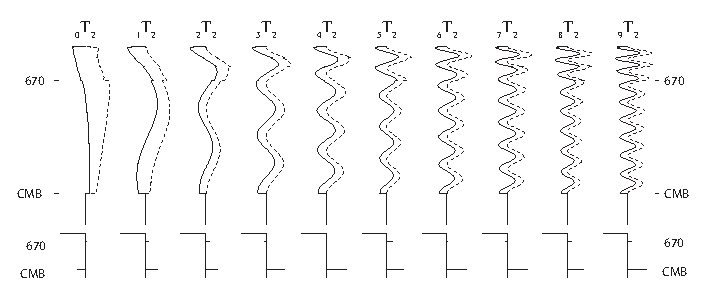
\includegraphics{../figures/chap09/fig01.eps}
}
\end{center}
\caption[torkernels1]{\label{9.fig.tor1}
二次环型模式~${}_0{\rm T}_2, \ldots,{}_9{\rm T}_2$~的~Fr\'{e}chet~积分核~$K_{\beta}$~({\em 虚线\/})~和~$K_{\raisebox{0.3 ex}{\scriptsize$\rho$}}^{\prime}$~({\em 虚线\/})~(位移~$W$~和牵引力~$T$~见图~\ref{fig:deg2modes})。纵轴为地球表面向下的深度;图中标明了~670 km~不连续面和核幔边界(CMB)的位置。图的下部显示了对上述三个主要边界位置的微扰的敏感度。向左和向右的“树枝”分别对应于负的和正的积分核$[K_s]^+_-$、$[K_{670}]^+_-$和$[K_b]^+_-$。每幅图都各自做了缩放,以使所有积分核的最大值相同。
}
\end{figure}
图~\ref{9.fig.tor1}~显示了前~10~个~$l=2$~次环型模式的积分核~$K_{\beta}$~和~$K_{\raisebox{0.3 ex}{\scriptsize$\rho$}}^{\prime}$。这些模式对整个地幔的剪切波速~$\beta$~和密度~$\rho$~的变化都有敏感性;这些振荡的径向“波长”大约是等价的单频~${\rm ScS}_{\rm SH}$~波的两倍。增加~$\beta$~总会使本征频率增加,因为所有环型模式都有$K_{\beta}\geq 0$。这也符合基本的物理直觉:如果波在地球内部传播得更快,那么由这些波的相长干涉而形成的振荡的音调一定会升高。另一方面,增加密度产生的影响可正可负,与深度有关。这与~(\ref{9.Guust})~式中要求的所有环形模式的$\int_b^s\rho K_{\raisebox{0.3 ex}{\scriptsize$\rho$}}^{\prime}\,dr=0$一致。正如我们已看到的,均匀的相对微扰~$\delta\hspace{-0.2 mm}\rho/\hspace{-0.3 mm}\rho$~没有任何的一阶效应;长波长微扰(比~$K_{\raisebox{0.3 ex}{\scriptsize$\rho$}}^{\prime}$~振荡更长)的影响也很小。要记住,这些结果
适用于横波速度保持不变时的密度变化;反之,如果刚度~$\mu$~保持不变,则~$\rho$~的增加总是使环型模式的本征频率下降,因为此时,相关的积分核处处为非正的:$K_{\rho}\leq 0$。
\begin{figure}[!b]
\begin{center}
\scalebox{0.95}{
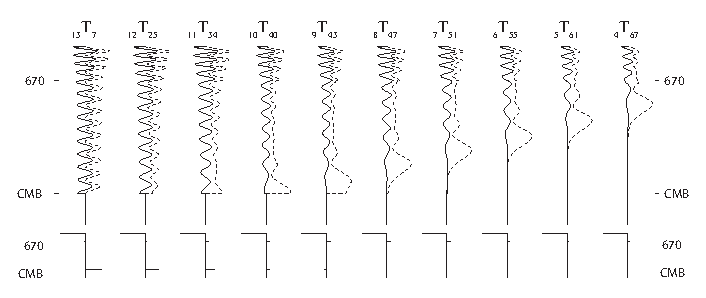
\includegraphics{../figures/chap09/fig02.eps}
}
\end{center}
\caption[torkernels2]{\label{9.fig.tor2}
与图~\ref{9.fig.tor1}~相同的一组本征频率大致均为~$\omega/2\pi\approx 14$~mHz~的~${\rm ScS}_{\rm SH}$~到~SH~模式(位移~$W$~和牵引力~$T$见图~\ref{fig:S&ScSmodes})。虚线和实线分别表示~$K_{\beta}$~和~$K_{\raisebox{0.3 ex}{\scriptsize$\rho$}}^{\prime}$。最右边的模式~${}_4{\rm T}_{67}$~基本上是第四个高阶勒夫波,它可以“感受”到约~1000~公里的深度。
}
\end{figure}
\begin{figure}[!b]
\begin{center}
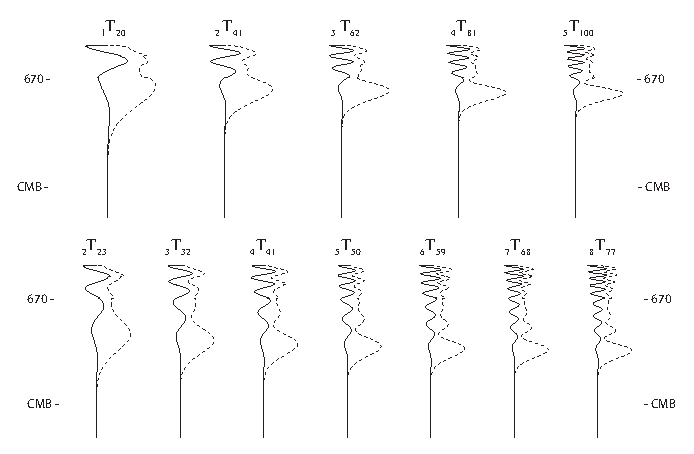
\includegraphics{../figures/chap09/fig03.eps}
\end{center}
\caption[torkernels3]{\label{9.fig.tor3}
一些~$n\approx l/20$~({\em 上图\/})~和~$n\approx l/10$~({\em 下图\/})~的环型模式~${}_n{\rm T}_l$~的~Fr\'{e}chet~积分核~$K_{\beta}$~({\em 虚线\/})~和~$K_{\raisebox{0.2 ex}{\scriptsize$\rho$}}^{\prime}$~({\em 实线\/})。相应的本征频率~${}_n\omega_l^{\rm T}$~为沿图~\ref{9.fig.tor4}~中的两条粗直线。
}
\end{figure}
\begin{figure}[!t]
\begin{center}
\scalebox{0.95}{
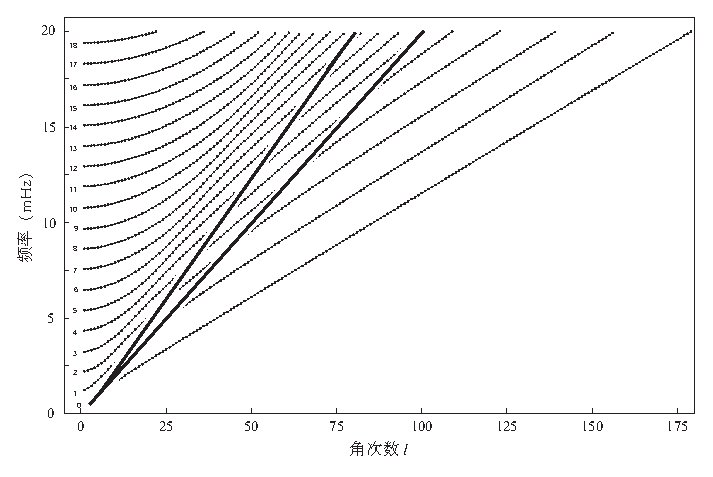
\includegraphics{../figures/chap09/fig04.eps}
}
\end{center}
\caption[torkernels4]{\label{9.fig.tor4}
显示图~\ref{9.fig.tor3}~中模式本征频率的环型模式频散图。较平和较陡的粗实线分别标示图~\ref{9.fig.tor3}中上图($n\approx l/20$)和下图($n\approx l/10$)的两组模式。
}
\end{figure}
这种微扰增加了地球内部每个体积元的惯性力,但保持恢复力不变。图~\ref{9.fig.tor1}~底部的“树枝”图显示了积分核~$[K_s]^+_-$、$[K_{670}]^+_-$~和~$[K_b]^+_-$,它们分别表示海底、670~km~不连续性和核幔边界的位置微扰的影响。海底高度的增加~$\delta\hspace{-0.1 mm}s>0$~会降低所有的环型模式的本征频率,而核幔边界半径的增加~$\delta b>0$~则会升高除基阶模式~${}_0{\rm T}_2$~以外所有模式的本征频率。这些结果也有一个简单的物理解释:这两个扰动分别扩大和缩小了等价~${\rm ScS}_{\rm SH}$~波所传播的地幔的体积。${}_0{\rm T}_2$~模式的本征频率的减小~$[K_b]^+_-<0$~不能通过这种仅在~$\om\rightarrow\infty$\vspace{-0.5mm}~极限下才严格成立的射线-模式二象性的推论来预测。

图~\ref{9.fig.tor2}~显示了一些本征频率近似均为~$\om/2\pi\approx 14$ mHz~的环型模式的~Fr\'{e}chet~积分核~$K_{\beta}$、$K_{\raisebox{0.3 ex}{\scriptsize$\rho$}}^{\prime}$~和~$[K_s]^+_-$、$[K_{670}]^+_-$、$[K_b]^+_-$。许多特征仍然很明显;特别要注意的是,对剪切波速度微扰的敏感度占主导地位且固有为正值~($K_{\beta}>0$),而对密度的依赖性则表现出均值为零的振荡$\int_b^s\rho K_{\raisebox{0.3 ex}{\scriptsize$\rho$}}^{\prime}\,dr=0$。最显著的新特征是在~$n\approx l/4$~时,能够“感觉到”核幔边界的~${\rm ScS}_{\rm SH}$~反射波等价模式
与感觉不到核幔边界的~SH~折返波等价模式之间的转换。SH~折返波等价模式的剪切波积分核~$K_{\beta}$~在折返半径附近有极大值,相长干涉的波在那里渡过的时间最长。在折返半径以下,微扰~$\delta\hspace{-0.2 mm}\beta$~和~$\delta\hspace{-0.2 mm}\rho$~以及核幔边界位置的微扰~$\delta b$~对~SH~等价模式本征频率的影响可以忽略不计。

图~\ref{9.fig.tor3}~显示了两组折返半径近似相同的环型模式的~Fr\'{e}chet~积分核~$K_{\beta}$~和~$K_{\raisebox{0.3 ex}{\scriptsize$\rho$}}^{\prime}$。相应的本征频率落在图~\ref{9.fig.tor4}~中所示环型模式频散图中的两条直线上。所有~$n\approx l/20$~的模式的~$K_{\beta}$~在~$h\approx 900$~km~处有极大值,而~$n\approx l/10$~的模式的~$K_{\beta}$~则在~$h\approx 1800$~km~处有极大值。这展示了我们将在第~12~章中更全面探讨的模式-射线二象性的一般原理:具有相同相速度~$\om/k\approx\om/(l+\half)$~的高频环型或球型模式是由射线参数~$p=(l+\half)/\om$~相同的、相长干涉的~SH~或~P-SV~体波组成的。

图~\ref{9.fig.spher1}~和~\ref{9.fig.spher2}~分别显示了基阶球型模式~${}_0{\rm S}_2$~至~${}_0{\rm S}_9$~和前九个径向模式~${}_n{\rm S}_0$~的~Fr\'{e}chet~积分核~$K_{\alpha}$、$K_{\beta}$、$K_{\raisebox{0.3 ex}{\scriptsize$\rho$}}^{\prime}$~以及~$[K_s]^+_-$、
$[K_{670}]^+_-$、$[K_b]^+_-$、$[K_c]^+_-$。
%%%
\begin{figure}
\begin{center}
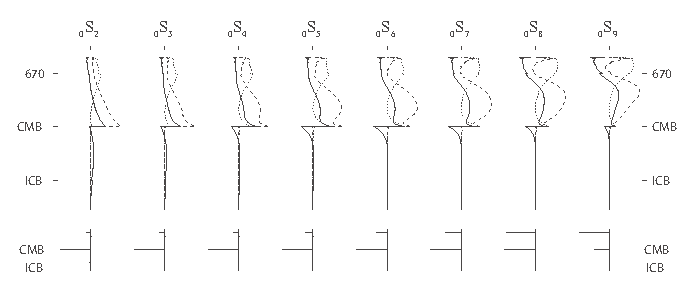
\includegraphics{../figures/chap09/fig05.eps}
\end{center}
\caption[spherkernels]{\label{9.fig.spher1}
基阶球型模式~${}_0{\rm S}_2, \ldots,{}_0{\rm S}_9$的~Fr\'{e}chet~积分核~$K_{\alpha}$~({\em 点线\/}),$K_{\beta}$~({\em 虚线\/})和~$K_{\raisebox{0.3 ex}{\scriptsize$\rho$}}^{\prime}$~({\em 实线\/})(橄榄球模式的位移~$U$、$V$~和牵引力~$R$、$S$~见图~\ref{fig:0S2})。纵轴是地球表面向下的深度,图中标明了~670~km~不连续面、核幔边界(CMB)和内核边界(ICB)的位置。图的下部显示了对海底和这三个界面位置的微扰的敏感度。向左和向右的“树枝”分别对应负的和正的积分核~$[K_s]^+_-$、$[K_{670}]^+_-$、$[K_b]^+_-$、$[K_c]^+_-$(从上到下)。每幅图都各自做了缩放,以使所有积分核的最大值相同。
}
\end{figure}
\begin{figure}
\begin{center}
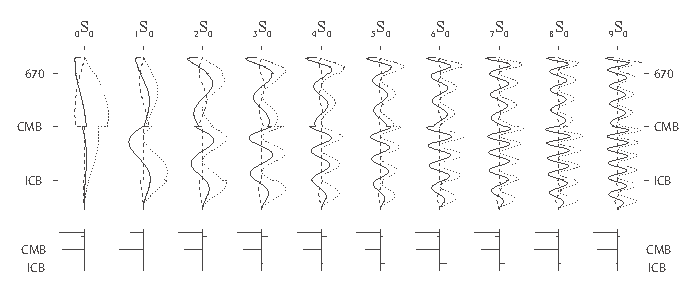
\includegraphics{../figures/chap09/fig06.eps}
\end{center}
\caption[radkernels]{\label{9.fig.spher2}
与图~\ref{9.fig.spher1}~相同的基阶和高阶径向模式~${}_0{\rm S}_0, \ldots,{}_9{\rm S}_0$~的~Fr\'{e}chet~积分核(位移~$U$~和牵引力~$R$~见图~\ref{fig:radeifs})。点线、虚线和实线分别表示~$K_{\alpha}$、$K_{\beta}$~和~$K_{\raisebox{0.3 ex}{\scriptsize$\rho$}}^{\prime}$。
}
\end{figure}
\begin{sidewaysfigure}
\centering
\rotatebox{270}
{
\scalebox{0.95}{
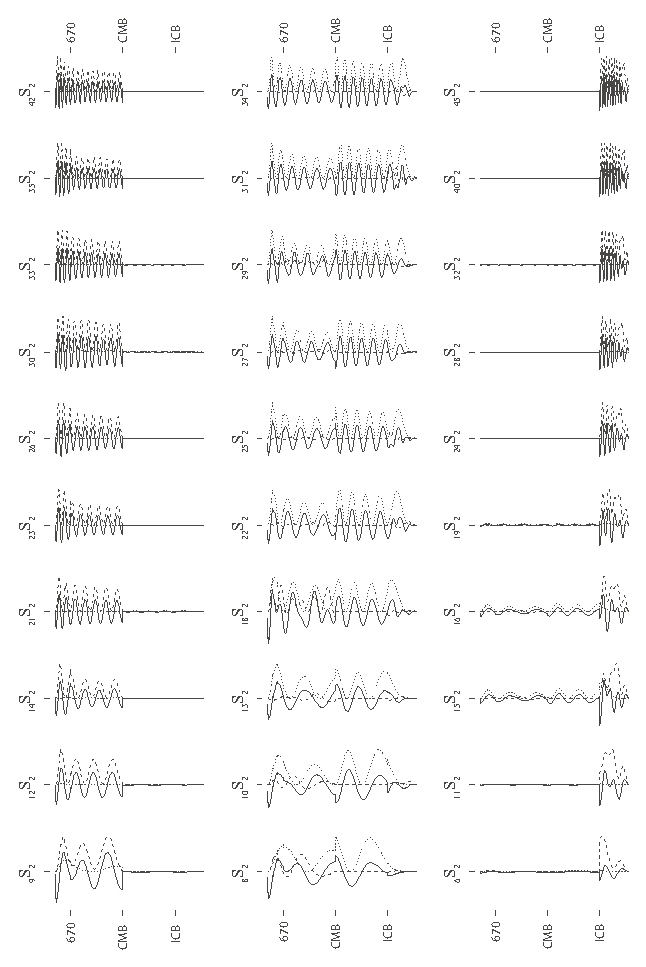
\includegraphics{../figures/chap09/fig07.eps}
}
}
\caption[ScS&J&PKIKPkernels]{
一些次数~$l=2$~的~${\rm ScS}_{\rm SV}$~模式~({\em 最上行\/})、PKIKP~模式~({\em 中间行\/})~和~${\rm J}_{\rm SV}$~模式~({\em 最下行\/})~的~Fr\'{e}chet~积分核~$K_{\alpha}$~({\em 点线\/})、$K_{\beta}$~({\em 虚线\/})~和~$K_{\rho}^{\prime}$~({\em 实线\/})。位移~$U$~和~$V$~在图~\protect\ref{fig:ScS&J&PKIKP}~中显示。每幅图都独立做了缩放,以使所有积分核的最大值相同。
}
\label{9.fig.spher3}
\end{sidewaysfigure}
“橄榄球”模式~${}_0{\rm S}_2$~的本征频率是所观测到的地球的最低频振荡,它依赖于整个地球的~$\alpha$、$\beta$~和~$\rho$;
\index{football mode}%
\index{fundamental mode!spheroidal}%
然而,它最明显的敏感度是对下地幔底部的剪切波速度。当我们沿基阶模式分支上升到~${}_0{\rm S}_9$~模式时,$K_{\beta}$~敏感度积分核的峰值也上移到大约~1500~km~深处,等价于一个很长周期(634~s)的瑞利波。基阶径向模式~${}_0{\rm S}_0$~对整个地球的两种波速和密度都很敏感,就像“橄榄球”模式一样;然而,如${}_9{\rm S}_0$~这样的高阶径向模则等价于径向传播的~PKIKP~波,主要对纵波速度~$\alpha$~敏感,正如预期的。积分核振荡的“波长”大约是单频~PKIKP~波的两倍。核幔边界半径的增加会缩短(较快的)地幔射线路径的长度,同时延长(较慢的)地核射线路径长度;从而导致~PKIKP~走时增加,并因此降低这些与其他~PKIKP~等价模式的本征频率。
\begin{figure}[!t]
\begin{center}
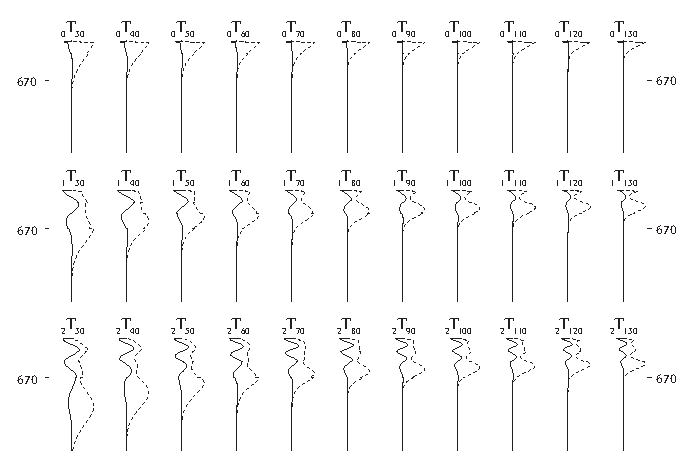
\includegraphics{../figures/chap09/fig08.eps}
\end{center}
\caption[Lovemodekernels]{\label{9.fig.Love}
沿基阶~({\em 最上行\/})、第一高阶~({\em 中间行\/})~和第二高阶~({\em 最下行\/})~勒夫波等价模式分支的~Fr\'{e}chet~积分核~$K_{\beta}$~({\em 虚线\/})~和~$K_{\raisebox{0.3 ex}{\scriptsize$\rho$}}^{\prime}$~({\em 实线\/})~的变化。纵轴从自由表面延伸到~1500~km~深度;图中标明了~670~km~间断的位置。位移~$W$~如图~\ref{fig:Lovemodes2}~所示。每幅图均做了独立缩放,以使~$K_{\beta}$~具有相同的最大值;实际上,基阶模式积分核大约是高阶模式积分核的三倍。
}
\end{figure}

图~\ref{9.fig.spher3}~中按模式类型比较了一些二次球型模式的体积~Fr\'{e}chet~积分核~$K_{\alpha}$、$K_{\beta}$、$K_{\raisebox{0.3 ex}{\scriptsize$\rho$}}^{\prime}$。其中${\rm ScS}_{\rm SV}$~等价模式与图~\ref{9.fig.tor1}~中的~${\rm ScS}_{\rm SH}$~环型模式类似的球型模式;
\index{ScS-equivalent mode}%
\index{mode!ScS-equivalent}%
它们的敏感度主要是对地幔中的剪切波速~$\beta$。PKIKP~等价模式与图~\ref{9.fig.spher2}~中的径向模式有相似特性;
\index{PKIKP-equivalent mode}%
\index{mode!PKIKP-equivalent}%
\enlargethispage{-0.5\baselineskip}
压缩波敏感核~$K_{\alpha}$~的“波长”从下地幔~($\alpha=13.7$~km/s)~到液态外核~($\alpha=8.1$~km/s)~有明显的特征变化,尤其是高频模式,如~${}_{31}{\rm S}_2$~和~${}_{34}{\rm S}_2$。最后,如预期的,${\rm J}_{\rm SV}$~等价模式主要是对固态内核中的剪切波速~$\beta$~敏感。
\index{J-equivalent mode}%
\index{mode!J-equivalent}%
所有这三种模式的密度积分核都较大,但都是振荡的,正负值大致相等,符合~$\int_0^a\rho K_{\raisebox{0.3 ex}{\scriptsize$\rho$}}^{\prime}\,dr=0$~的约束条件,因而长波长的密度微扰~$\delta\hspace{-0.2 mm}\rho$~的影响很小。
\begin{figure}[!t]
\begin{center}
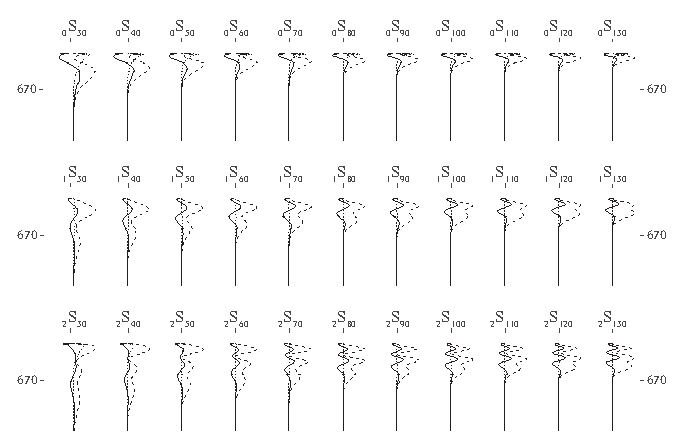
\includegraphics{../figures/chap09/fig09.eps}
\end{center}
\caption[Raymodekernels]{\label{9.fig.Ray}
沿基阶~({\em 最上行\/})、第一高阶~({\em 中间行\/})~和第二高阶~({\em 最下行\/})~瑞利波等价模式分支的~Fr\'{e}chet~积分核~$K_{\alpha}$~({\em 点线\/}),$K_{\beta}$~({\em 虚线\/})~和~$K_{\raisebox{0.3 ex}{\scriptsize$\rho$}}^{\prime}$~({\em 实线\/})~的变化。纵轴从自由表面延伸到~1500~km~深度;图中标明了~670~km~间断面的位置。位移~$U$~和~$V$~如图~\ref{fig:fundsphmodes}~所示。每幅图均做了独立缩放,以使~$K_{\beta}$~具有相同的最大值;实际上,基阶模式积分核大约是高阶模式积分核的三倍。
}
\end{figure}

图~\ref{9.fig.Love}~和~\ref{9.fig.Ray}~显示了沿基阶和前两个高阶面波频散分支的各向同性~Fr\'{e}chet~积分核~$K_{\alpha}$、$K_{\beta}$~和~$K_{\raisebox{0.3 ex}{\scriptsize$\rho$}}^{\prime}$~的变化。
\index{surface-wave equivalent mode}%
\index{mode!surface-wave-equivalent}%
\enlargethispage{-0.5\baselineskip}
很明显,勒夫和瑞利模式主要的敏感度是对上地幔剪切波速~$\beta$~的变化。基阶瑞利模式~${}_0{\rm S}_l$~对压缩波速~$\alpha$~有微弱的依赖性;但~$\alpha$~对高阶模式~${}_1{\rm S}_l$~和~${}_2{\rm S}_l$~的影响几乎可以忽略。基阶勒夫模式~${}_0{\rm T}_l$~的剪切波敏感核~$K_{\beta}$~在约~$0.1\!-\!0.2\,\lambda$~深处达到最大值,其中~$\lambda=2\pi a/k$~为等价行波的波长。相应的基阶瑞利模式敏感度的最大值要深得多,约为~$0.3\!-\!0.4\,\lambda$。
\begin{figure}[!t]
\begin{center}
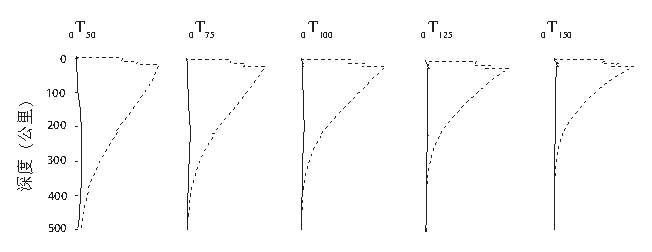
\includegraphics{../figures/chap09/fig10.eps}
\end{center}
\caption[anisotropic kernels 1]{
\label{fig:9.10}
沿基阶环型模式分支的横向各向同性~Fr\'{e}chet~积分核~$K_{\beta_{\rm v}}$~({\em 实线\/})~和~$K_{\beta_{\rm h}}$~({\em 虚线\/})~ 的变化。每幅图均做了独立缩放,以使~$K_{\beta_{\rm h}}$~具有相同的最大值。
}
\end{figure}
\begin{figure}[!b]
\begin{center}
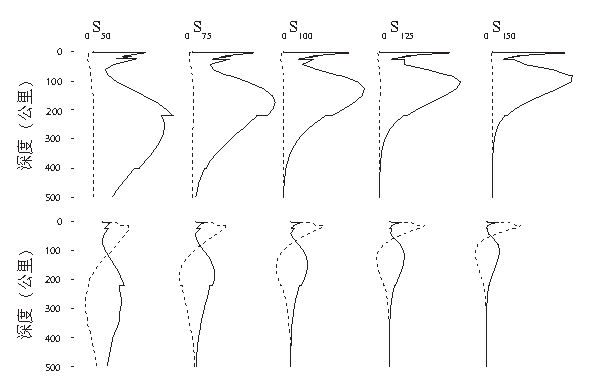
\includegraphics{../figures/chap09/fig11.eps}
\end{center}
\caption[anisotropic kernels 2]{
\label{fig:9.11}
沿基阶球型模式分支的横向各向同性~Fr\'{e}chet~积分核的变化。上行显示了剪切波速积分核~$K_{\beta_{\rm v}}$~({\em 实线\/})和~$K_{\beta_{\rm h}}$~({\em 虚线\/})。下行显示了压缩波积分核~$K_{\alpha_{\rm v}}$~({\em 实线\/})~和~$K_{\alpha_{\rm h}}$~({\em 虚线\/})。每幅图均做了独立缩放,以使~$K_{\beta_{\rm v}}$~具有相同的最大值。
}
\end{figure}
与基阶模式相比,${}_1{\rm T}_l$、${}_2{\rm T}_l$~和~${}_1{\rm S}_l$、${}_2{\rm S}_l$~这些高阶模式对深部的变化~$\delta\hspace{-0.2 mm}\beta$~更为敏感。因此,周期为97秒的~${}_0{\rm S}_{100}$~模式对~250~km~以下的敏感度非常有限,而周期大致相同的第一和第二高阶模式~${}_1{\rm S}_{68}$~和~${}_2{\rm S}_{56}$~所能“感觉”到的深度远在~670~km~间断面以下。在第~\ref{11.sec.cpert}~节中,我们建立单频面波相速度微扰~$\delta c$~与等价自由振荡的本征频率微扰~$\delta\om$~之间的关系。

图~\ref{fig:9.10}~和~\ref{fig:9.11}~显示了沿横向各向同性~PREM~的~${}_0{\rm T}_l$~和~${}_0{\rm S}_l$~分支的~Fr\'{e}chet~积分核~$K_{\beta_{\rm v}}$、$K_{\beta_{\rm h}}$~和~$K_{\alpha_{\rm v}}$、$K_{\alpha_{\rm h}}$~的径向变化。基阶环型的本征频率对垂直传播的剪切波速~$\beta_{\rm v}$~的微扰几乎完全没有敏感度;另一方面,基阶球型的本征频率主要对~$\beta_{\rm v}$~敏感,而几乎与水平传播的剪切波速~$\beta_{\rm h}$~无关。正是$\beta_{\rm h}$~和~$\beta_{\rm v}$~的这种近乎完全的“解耦”,使得横向各向同性的上地幔模型能够拟合无法协调的勒夫和瑞利基阶模式本征频率的观测值。${}_0{\rm S}_l$~模式对上地幔的两个压缩波速~$\alpha_{\rm v}$~和~$\alpha_{\rm h}$~的微扰也有微弱的敏感度。
\index{Fr\'{e}chet kernel|)}%
\index{kernel!Fr\'{e}chet|)}%

%\section{Anelasticity and Attenuation}
\section{非弹性和衰减}
\index{anelasticity|(}%
\index{attenuation|(}%
\label{section:anelas}

我们在第六章已经看到,各向同性非弹性可以通过将~$\delta\hspace{-0.1 mm}\kappa$~和~$\delta\hspace{-0.2 mm}\mu$~用与频率相关的复数微扰来处理。我们略微变更一下符号,自此分别用~$\kappa_0$~和~$\mu_0$~表示扰动前的~SNREI~地球模型的不可压缩性和刚性。下角标~0~表示它们被视为是对参考或基准频率~$\om_0$~下的地球弹性特性的适当描述;PREM~模型的参考频率是~1~Hz,即$\om_0=2\pi$~rad/s。我们考虑如下形式的无穷小非弹性扰动
\eq \label{9.anel1}
\kappa_0\rightarrow\kappa_0+\delta\hspace{-0.1 mm}\kappa(\om)
+i\kappa_0Q_{\kappa}^{-1},
\en
\eq \label{9.anel2}
\mu_0\rightarrow\mu_0+\delta\hspace{-0.2 mm}\mu(\om)
+i\mu_0Q_{\mu}^{-1},
\en
式中~$Q_{\kappa}$~和~$Q_{\mu}$~分别为体积和剪切品质因子,假设它们与频率无关。
\index{Q@{\em Q}!bulk}%
\index{Q@{\em Q}!shear}%
\index{quality factor!bulk}%
\index{bulk quality factor}%
\index{shear quality factor}%
\index{quality factor!shear}%
微扰前本征频率为正的~$\om$~的简正模式所“感觉到”的实数的不可压缩性和刚性微扰为:
\eq \label{9.anel3}
\delta\hspace{-0.1 mm}\kappa(\om)=\delta\hspace{-0.1 mm}\kappa_0
+\twoinvpi\kappa_0 Q_{\kappa}^{-1}\ln(\om\hspace{-0.2 mm}/\hspace{-0.2 mm}\om_0),
\en
\eq \label{9.anel4}
\delta\hspace{-0.2 mm}\mu(\om)=\delta\hspace{-0.2 mm}\mu_0
+\twoinvpi\mu_0Q_{\mu}^{-1}\ln(\om\hspace{-0.2 mm}/\hspace{-0.2 mm}\om_0),
\en
其中第一项为在参考频率~$\om_0$~下的扰动,第二项来自非弹性频散。

我们将任一振荡的正的本征频率的复数微扰写为如下形式
\eq \label{9.anel5}
\om\rightarrow\om+\delta\om_0+\delta\om_{\rm d}+i\gamma,
\en
其中~$\delta\om_0$~表示在参考频率下的微扰的影响,$\delta\om_{\rm d}$~表示额外的对数频散效应。
\index{logarithmic dispersion}%
\index{dispersion!logarithmic}%
$\gamma$~为衰减率,它与模式的品质因子~$Q$~的关系为:
\index{decay rate}%
\index{Q@{\em Q}!of a mode}%
\index{quality factor!of a mode}%
\eq \label{9.anel6}
\gamma=\half\om Q^{-1}.
\en
要得到~$\delta\om_{\rm 0}$、$\delta\om_{\rm d}$~和~$\gamma$~这三个扰动,我们将~(\ref{9.anel1})--(\ref{9.anel6})~代入~(\ref{eq:9.delomiso}),并相关项做适当整理。令虚部相等可以得到品质因子的倒数
\eq \label{9.anel7}
Q^{-1}=2\om^{-1}\int_0^a[(\kappa_0K_{\kappa})Q_{\kappa}^{-1}
+(\mu_0K_{\mu})Q_{\mu}^{-1}]\,dr.
\en
如果我们的目的只是要计算无穷小非弹性对~SNREI~本征频率~$\om$~的影响,我们令~$\delta\hspace{-0.1 mm}\kappa_0$~和~$\delta\hspace{-0.2 mm}\mu_0$~为零,此时有~$\delta\om_0=0$,以及
\eq \label{9.delwdisp}
\delta\om_{\rm d}=\invpi\om Q^{-1}
\ln(\om\hspace{-0.2 mm}/\hspace{-0.2 mm}\om_0).
\en
更一般地,我们可以将~$\delta\hspace{-0.1 mm}\kappa_0$~和~$\delta\hspace{-0.2 mm}\mu_0$~连同~$\delta\hspace{-0.2 mm}\rho$~和~$\delta\hspace{-0.1 mm}d$~一并视为参考~SNREI~地球模型的特定微扰。这导致实数本征频率的一个附加的微扰,由~(\ref{eq:9.delomiso})~给定,只要把~$\delta\om$、$\delta\hspace{-0.1 mm}\kappa$~和~$\delta\hspace{-0.2 mm}\mu$~用~$\delta\om_0$、$\delta\hspace{-0.1 mm}\kappa_0$~和~$\delta\hspace{-0.2 mm}\mu_0$~替换。(\ref{9.delwdisp})~式表示的频散校正对于所有微扰前本征频率小于基准频率~$\om<\om_0$~的自由振荡为负值,而对于所有~$\om>\om_0$~的振荡则为正值。在物理上这是合理的,因为一个频率更低或更高的这种模式所“感觉到”的地球比参考~SNREI~地球模型
具有更高或更低的柔度。

一个弹性参数为~$C_0$、$A_0$、$L_0$、$N_0$~和~$F_0$~的横向各向同性弹性地球模型,如果其“等效”不可压缩性~$\kappa_0=\ninth(C_0+4A_0-4N_0+4F_0)$~和刚度~$\mu_0=\fifteenth(C_0+A_0+6L_0+5N_0-2F_0)$为~(\ref{9.anel1})--(\ref{9.anel4})~所示的与频率相关的复数参数替换,则变成各向同性非弹性的。$C_0^{\prime}=C_0-\kappa_0-\fourthirds\mu_0$、$A_0^{\prime}=A_0-\kappa_0-\fourthirds\mu_0$、$L_0^{\prime}=L_0-\mu_0$、$N_0^{\prime}=N_0-\mu_0$~和~$F_0^{\prime}=F_0-\kappa_0+\twothirds\mu_0$~这五个“纯”各向异性参数被视为实数且与频率无关。一个简正模式的品质因子倒数~$Q^{-1}$~仍由~(\ref{9.anel7})~式给定;唯一的差别是位移本征函数~$U$、$V$~和~$W$~均属于横向各向同性参考模型。在参考频率~$\om_0$~下地球结构的任何微扰都会造成一个由~(\ref{eq:9.delomti})~式给定的附加实数本征频率微扰,其中~$\delta\om$
、$\delta C$、$\delta\hspace{-0.2 mm}A$、$\delta\hspace{-0.1 mm}L$、$\delta\hspace{-0.1 mm}N$~和~$\delta\hspace{-0.1 mm}F$~由~$\delta\om_0$、$\delta C_0$、$\delta\hspace{-0.2 mm}A_0$、$\delta\hspace{-0.1 mm}L_0$、$\delta\hspace{-0.1 mm}N_0$~和~$\delta\hspace{-0.1 mm}F_0$~所取代。

总之,一个球对称、无自转、非弹性、各向同性(SNRAI)的地球模型完全由五个恒正的半径的函数---$\kappa_0$、$\mu_0$、$\rho$、$Q_{\kappa}$~和~$Q_{\mu}$---表述,而横向各向同性模型则由八个半径的函数---$C_0$、$A_0$、$L_0$、$N_0$、$F_0$、$\rho$、$Q_{\kappa}$~和~$Q_{\mu}$---给定,其中下角标零表示它们是对应于参考或基准频率~$\om_0$~的。(\ref{9.anel7})~式为利用观测的衰减率~$\gamma$~或地球自由振荡的品质因子~$Q$~来反演地球内固有衰减的径向变化提供了理论基础。体积和剪切品质因子倒数~$Q_{\kappa}^{-1}$~和~$Q_{\mu}^{-1}$~的这一反演问题以其线性而著称。非弹性~Fr\'{e}chet~积分核有一个直观的物理解释:$2\om^{-1}r^{-2}(\kappa_0K_{\kappa})$~和~$2\om^{-1}r^{-2}(\mu_0K_{\mu})$~是每个模式的压缩和剪切能量密度占比(因子$r^{-2}$~源于我们所约定的在~Fr\'{e}chet~积分核关系中的微分元素是~$dr$,而不是~$r^2dr$)。当固有品质因子仅微弱地依赖于半径时,(\ref{9.anel7})~式退化为
\eq
Q^{-1}\approx f_{\kappa}Q_{\kappa}^{-1}+
f_{\mu}Q_{\mu}^{-1},
\en
其中~$f_{\kappa}=2\om^{-1}\int_0^a(\kappa_0K_{\kappa})\,dr$~和~$f_{\mu}=2\om^{-1}\int_0^a(\mu_0K_{\mu})\,dr$~是净能量占比。很明显,体积衰减只会对具有较大压缩能量占比的模式(即径向和其他~PKIKP~等价球型模式)产生明显的影响。环型模式没有压缩,因而它们的阻尼仅依赖于~$Q_{\mu}$;如果剪切衰减与半径几乎无关,那么所有环型模式将有几乎相同的品质因子~$Q\approx Q_{\mu}$。

有两种策略可以用来反演观测到的地球的本征频率~$\om$~来得到拟合的最佳的球对称弹性结构~$\kappa_0$、$\mu_0$~和~$\rho$,或者一般的~$C_0$、$A_0$、$L_0$、$N_0$、$F_0$~和~$\rho$。每种方法都可以如前所述地计算微扰前的完全弹性、无频散的参考地球模型的本征频率,并通过在反演之前减去~$\delta\om_d$~来对残差~$\om_{\rm meas}
-\om_{\rm calc}$做频散“校正”,或者在从径向标量方程中求解~$\om$~和~$U$、$V$、$W$~时直接考虑频散的影响。后者是大多数应用中首选的做法;{\tt MINEOS\/}和{\tt OBANI\/}都考虑了物理频散,
\index{MINEOS@\texttt{MINEOS}}%
\index{OBANI@\texttt{OBANI}}%
因而所有简正模式所“感觉到”的都是在微扰前的振荡频率~$\om$~下的实数各向同性弹性参数~$\kappa_0[1+\twoinvpi Q_{\kappa}^{-1}\ln
(\om\hspace{-0.2 mm}/\hspace{-0.2 mm}\om_0)]$~和~$\mu_0[1+\twoinvpi Q_{\mu}^{-1}
\ln(\om\hspace{-0.2 mm}/\hspace{-0.2 mm}\om_0)]$。要注意的是,无论以何种方法计算,对频散的校正依赖于衰减模型~$Q_{\kappa}$~和~$Q_{\mu}$。最好是将参考频率~$\om_0$~选在简正模式频带的中心附近,以便将这些参数不确定性的影响降到最低。从这一点考虑~PREM~的~1~Hz~参考频率并不理想,因为它导致许多基阶模式~${}_0{\rm S}_l$~和~${}_0{\rm T}_l$~的频散校正~$\delta\om_{\rm d}$~高达其观测误差的十倍以上~(Widmer \citeyear{widmer91})。

对于某些应用,用压缩和剪切波速来参数化非弹性比用不可压缩性和刚度会更方便。此时参考地球模型是由各向同性速度~$\alpha_0=[(\kappa_0+\fourthirds\mu_0)/\hspace{-0.2 mm}\rho]^{1/2}$~和~$\beta_0=(\mu_0/\hspace{-0.2 mm}\rho)^{1/2}$表述的,我们考虑如下形式的复数微扰
\eq
\alpha_0\rightarrow\alpha_0+\delta\hspace{-0.1 mm}\alpha(\om)
+\half i\alpha_0Q_{\alpha}^{-1},
\en
\eq
\beta_0\rightarrow\beta_0+\delta\hspace{-0.2 mm}\beta(\om)
+\half i\beta_0Q_{\beta}^{-1}.
\en
P~波和~S~波的品质因子~$Q_{\alpha}$~和~$Q_{\beta}$~与体积和剪切品质因子$Q_{\kappa}$和$Q_{\mu}$之间的关系为
\index{Q@{\em Q}!compressional-wave}%
\index{Q@{\em Q}!shear-wave}%
\index{quality factor!compressional-wave}%
\index{quality factor!shear-wave}%
\eq
Q_\alpha^{-1}=(1-\fourthirds
\beta_0^2/\alpha_0^2)Q_\kappa^{-1}
+\fourthirds(\beta_0^2/\alpha_0^2)Q_\mu^{-1},
\en
\eq
Q_\beta^{-1}=Q_\mu^{-1}.
\en
在参考频率~$\om_0$~下波速的实数微扰由类似于~(\ref{9.anel3})--(\ref{9.anel4})~的关系给定:
\eq
\delta\hspace{-0.1 mm}\alpha(\om)=\delta\hspace{-0.1 mm}\alpha_0
+\invpi\alpha_0 Q_{\alpha}^{-1}\ln(\om\hspace{-0.2 mm}/\hspace{-0.2 mm}\om_0),
\en
\eq
\delta\hspace{-0.2 mm}\beta(\om)=\delta\hspace{-0.2 mm}\beta_0
+\invpi\beta_0 Q_{\beta}^{-1}\ln(\om\hspace{-0.2 mm}/\hspace{-0.2 mm}\om_0).
\en
微扰~$\delta\om_0$~是用参考频率~$\om_0$~下的波速微扰由~(\ref{eq:9.delomiso2})~式给定,其中~$\delta\om$、$\delta\hspace{-0.1 mm}\alpha$~和~$\delta\hspace{-0.2 mm}\beta$~为~$\delta\om_0$、$\delta\hspace{-0.1 mm}\alpha_0$~和~$\delta\hspace{-0.2 mm}\beta_0$~取代,而自由振荡的品质因子倒数~$Q^{-1}$~可以用~$Q_{\alpha}^{-1}$~和~$Q_{\beta}^{-1}$~写为如下形式
\eq \label{9.anel9}
Q^{-1}=\om^{-1}\int_0^a[(\alpha_0K_{\alpha})Q_{\alpha}^{-1}
+(\beta_0K_{\beta})Q_{\beta}^{-1}]\,dr,
\en
其中~$K_{\alpha}=2\rho\alpha_0K_{\kappa}$~和~$K_{\beta}
=2\rho\beta_0(K_{\mu}-\fourthirds K_{\kappa})$。(\ref{9.anel9})~式可以用于反演~P~波和~S~波的品质因子~$Q_{\alpha}$~和~$Q_{\beta}$~的径向变化,与用~(\ref{9.anel7})~反演体积和剪切品质因子~$Q_{\kappa}$~和~$Q_{\mu}$~的做法一样。

%\section{\textit{Q} Kernels, Measurements and Models}
\section{\textit{Q}~的敏感核、测量和模型}
\index{kernel!{\em Q}|(}%
\index{Q@{\em Q} kernel|(}%
\index{Fr\'{e}chet kernel!anelastic|(}%

\begin{figure}[!b]
\begin{center}
\scalebox{0.96}{
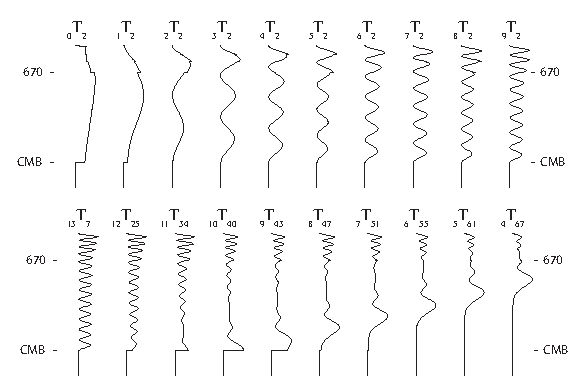
\includegraphics{../figures/chap09/fig12.eps}
}
\end{center}
\caption[Qkernels1]{\label{9.fig.Qkern1}
二次环型模式~${}_0{\rm T}_2, \ldots,{}_9{\rm T}_2$({\em 上行\/})和一组本征频率大致均为~$\omega/2\pi\approx 14$~mHz~的~${\rm ScS}_{\rm SH}$~至~SH~模式({\em 下行\/})的非弹性~Fr\'{e}chet~敏感核~$\mu_0K_{\mu}$。纵轴是地球表面向下的深度,图中标明了~670~km~不连续面和核幔边界~(CMB)~的位置。(\ref{9.anel7})~式中的常数因子~$2\omega^{-1}$~无关紧要,因为每个模式都做了独立缩放;$\mu_0K_{\mu}$~的最大值相同。弹性~Fr\'{e}chet~敏感核~$K_{\beta}$~和~$K_{\raisebox{0.3 ex}{\scriptsize$\rho$}}^{\prime}$见图~9.1~和~图9.2。
}
\end{figure}

图~\ref{9.fig.Qkern1}~显示了一组有代表性的环型模式的非弹性~Fr\'{e}chet~敏感核~$\mu_0K_{\mu}$。其中上行展示前十个二次模式~${}_n{\rm T}_2$,下行展示几个本征频率几乎相等的从~${\rm ScS}_{\rm SH}$~到~SH~过渡的模式。对~$Q_{\mu}^{-1}$~变化的敏感度在等价~SH~波的折返点附近达到最大值;下行中的~SH~等价模式的折返点在核幔边界与~670~km~深度之间的下地幔。图~\ref{9.fig.Qkern2}~显示了几个~$l=2$~次的球型振荡的敏感核~$\kappa_0K_{\kappa}$~和~$\mu_0K_{\mu}$。如预期的,${\rm ScS}_{\rm SV}$~等价模式主要对地幔中的~$Q_{\mu}^{-1}$~敏感,
\index{ScS-equivalent mode}%
\index{mode!ScS-equivalent}%
PKIKP~模式对整个地球的~$Q_{\kappa}^{-1}$~和~$Q_{\mu}^{-1}$~都敏感,
\index{PKIKP-equivalent mode}%
\index{mode!PKIKP-equivalent}%
而~${\rm J}_{\rm SV}$~模式对固态内核内的~$Q_{\mu}^{-1}$~敏感。
\index{J-equivalent mode}%
\index{mode!J-equivalent}%
最后,在图~\ref{9.fig.Qkern3}~和~图\ref{9.fig.Qkern4}~中,我们显示了沿基阶和两个最低频的高阶分支~${}_0{\rm T}_l$、${}_1{\rm T}_l$、${}_2{\rm T}_l$~和~${}_0{\rm S}_l$、${}_1{\rm S}_l$、${}_2{\rm S}_l$~上~$\kappa_0K_{\kappa}$~和~$\mu_0K_{\mu}$~的变化。这些面波等价模式的衰减受到上地幔剪切衰减~$Q_{\mu}^{-1}$~的强烈影响。
\index{surface-wave equivalent mode}%
\index{mode!surface-wave equivalent}%
\begin{figure}[!t]
\begin{center}
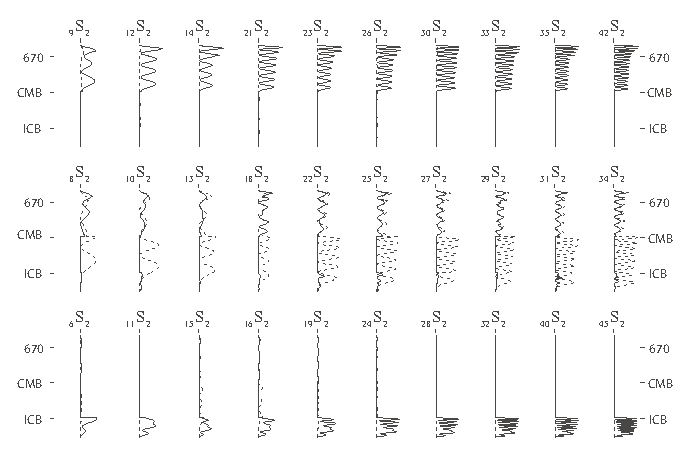
\includegraphics{../figures/chap09/fig13.eps}
\end{center}
\caption[Qkernels2]{\label{9.fig.Qkern2}
一些~$l=2$~次~${\rm ScS}_{\rm SV}$~模式~({\em 最上行\/})、PKIKP~模式~({\em 最上行\/})~和~${\rm J}_{\rm SV}$~模式~({\em 最上行\/})~的非弹性~Fr\'{e}chet~敏感核~$\kappa_0K_{\kappa}$~({\em 虚线\/})~和~$\mu_0K_{\mu}$~({\em 实线\/})。纵轴是地球表面向下的深度,图中标明了~670~km~不连续面、核幔边界~(CMB)~和内核边界~(ICB)~的位置。弹性~Fr\'{e}chet~敏感核~$K_{\alpha}$、$K_{\beta}$~和~$K_{\raisebox{0.3 ex}{\scriptsize$\rho$}}^{\prime}$~见图~9.7。
}
\end{figure}
低频勒夫和瑞利模式能比高频模式“感觉”到地球更深部的非弹性,同时,高阶模式能够“感觉到”的比基阶模式更深。如前所述,所有这些模式的敏感核~$Q_{\kappa}^{-1}$~和~$Q_{\mu}^{-1}$~也可以被视为压缩和剪切能量密度图---要记住它们是用半径而不是体积加权的。

自由振荡简正模式的衰减率~$\gamma$~可以直接用延时法对地震后观测到的对数振幅变化的直线拟合来测量。另外,也可以在频率域用洛伦兹谱峰函数拟合观测到的共振谱峰来同时测量一个孤立模式的频率~$\om$、品质因子~$Q$~和复数的激发振幅。无论使用哪种方法,有两个原因使得汇集一组高质量、无偏的~$Q$~数据比较困难。首先是单纯的统计效应:$Q$的最小二乘估计在本质上比~$\om$~的估计更不确定,因为后者的确定等同于寻找过零点,而前者的确定相当于估计衰减到~$e^{-1}$~的时间。
\begin{figure}[!t]
\begin{center}
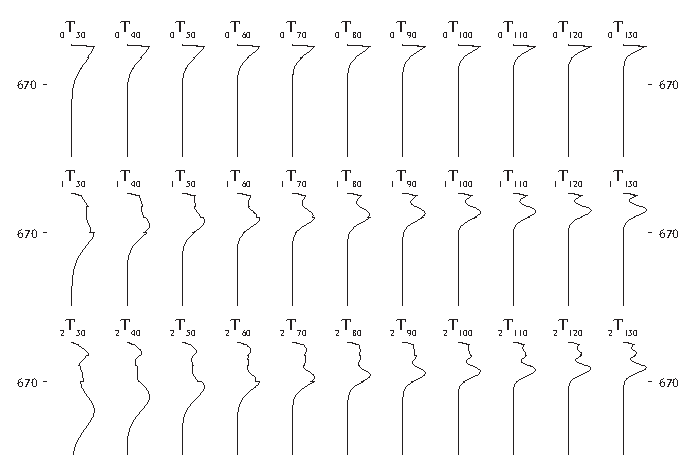
\includegraphics{../figures/chap09/fig14.eps}
\end{center}
\caption[Qkernels3]{\label{9.fig.Qkern3}
沿基阶~({\em 最上行\/})、第一高阶~({\em 中间行\/})~和第二高阶~({\em 最下行\/})~勒夫波等价模式分支的非弹性~Fr\'{e}chet~敏感核~$\mu_0K_{\mu}$~的变化。纵轴从自由表面延伸至~1500~km~深度;图中标明了~670~km~不连续面的位置。弹性~Fr\'{e}chet~敏感核~$K_{\beta}$~和~$K_{\raisebox{0.3 ex}{\scriptsize$\rho$}}^{\prime}$~见图~9.8。
}
\end{figure}
衰减率~$\gamma=\half\om Q^{-1}$~的相对标准差比频率的相对标准差大~$2Q$~倍;由于~$Q$~的典型值介于~$10^2$~和~$10^3$,衰减的测量总是会比本征频率的测量精度低~200--2000~倍~(Dahlen \citeyear{dahlen82})。其次,更重要的是,衰减数据受到由于地球自转、椭率和横向不均匀性所引起的分裂的污染;每个多态模式~${}_n{\rm S}_l$~或~${}_n{\rm T}_l$~中~$2l+1$~个间隔密集的单态模式的叠加导致了时间域中的差频和频率域中的峰值偏移和扭曲。由于这种分裂,未经处理的单台衰减测量没有任何规律性的地理分布(Smith \& Masters \citeyear{smith&masters89}),而频谱叠加测量得到的~$Q$~值会偏低~20--40\% (Widmer \citeyear{widmer91})。${}_0{\rm S}_l$~和~${}_0{\rm T}_l$~这些模式的衰减也可以通过测量等价的基阶瑞利和勒夫波随{\em 距离\/}的衰减率来研究(见第~\ref{sec.11.resp})~节)。
\begin{figure}[!t]
\begin{center}
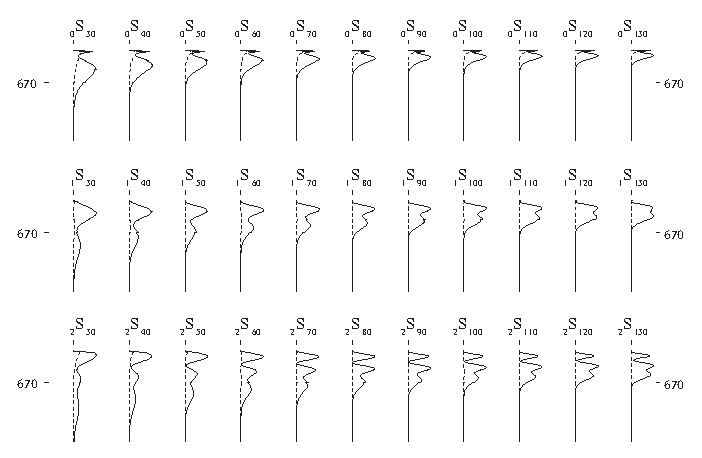
\includegraphics{../figures/chap09/fig15.eps}
\end{center}
\caption[Qkernels4]{\label{9.fig.Qkern4}
沿基阶({\em 最上行\/})、第一高阶({\em 中间行\/})和第二高阶({\em 最下行\/})瑞利波等价模式分支的非弹性~Fr\'{e}chet~敏感核~$\kappa_0K_{\kappa}$({\em 虚线\/})和~$\mu_0K_{\mu}$({\em 实线\/})的变化。纵轴从自由表面延伸至~1500~km~深度;图中标明了~670~km~不连续面的位置。弹性~Fr\'{e}chet~敏感核~$K_{\alpha}$、$K_{\beta}$~和~$K_{\raisebox{0.3 ex}{\scriptsize$\rho$}}^{\prime}$~见图~9.9。
}
\end{figure}
这种行波的测量也受到横向不均匀性的干扰,在第~16~章我们会讨论到,地球表面射线束的聚焦和焦散会引起振幅的几何变化。

径向模式~${}_n{\rm S}_0$~被视为一个明显的例外;
\index{radial mode}%
\index{Q@{\em Q}!radial mode}%
\index{quality factor!radial mode}%
\index{attenuation!radial mode}%
它们的本征频率是非简并的,所以没有任何分裂。此外,这些振荡在地球表面的所有地点都有相同的相位和振幅;因此,即使对震源位置或震源机制一无所知,也可将来自许多台站的数据进行叠加。图~\ref{9.fig.4S0}~显示了~1994~年~6~月~9~日玻利维亚深源地震后一些~${}_4{\rm S}_0$~模式的记录;
\index{Bolivia 1994 earthquake}%
Durek \& Ekstr\"{o}m
(\citeyear{durek&ekstrom95})~使用该数据测量了这一模式以及另外五个径向高阶模式的品质因子。基阶径向模式~${}_0{\rm S}_0$~没有被玻利维亚地震很好地激发;但是,Riedesel, Agnew, Berger \& Gilbert~(\citeyear{riedesel&al80})~在~1977~年~8~月~17~日印度尼西亚Sumbawa地震之后对该模式和第一径向高阶模式~${}_1{\rm S}_0$~的衰减进行了测量。
\index{Sumbawa 1977 earthquake}%
\begin{figure}[!t]
\begin{center}
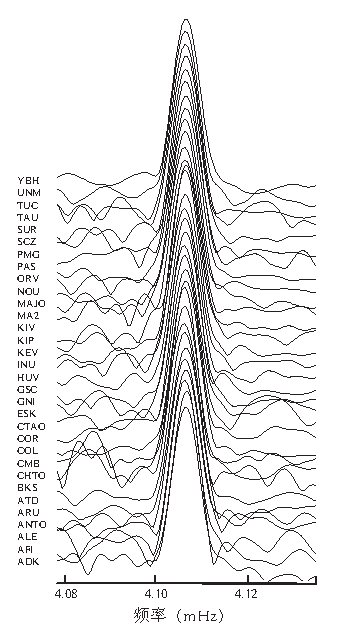
\includegraphics{../figures/chap09/fig16.eps}
\end{center}
\caption[Qkernels4]{\label{9.fig.4S0}
1994~年~6~月~9~日玻利维亚深源地震后~${}_4{\rm S}_0$~共振谱峰附近的单台频谱~(Durek \& Ekstr\"{o}m \citeyear{durek&ekstrom95})。在所有台站所显示的量都是~50--80~小时记录加~Hann~时窗以后的傅立叶变换绝对值;台站代号显示在左侧。主峰两侧的波动源于噪声(由~G. Ekstr\"{o}m~提供)。
}
\end{figure}
基阶径向模式的缓慢衰减~($Q\approx 5700$)~使得需要分析三个月的连续地震数据!这种异常高~$Q$~值的原因是~${}_0{\rm S}_0$~的低剪切能含量~($f_{\mu}=0.03$)。径向高阶的剪切能占比要大~5~到~6~倍(见表~8.2),因而品质因子相应较低;例如,${}_1{\rm S}_0$~有~$Q\approx 2000$,而~${}_4{\rm S}_0$~有~$Q\approx 1200$。径向振荡很长的持续时间使我们可以非常精确地测量它们的本征频率;确实,${}_0{\rm S}_0$~和~${}_1{\rm S}_0$~模式的频率~$0.814664\pm 0.000004$~mHz~和~$1.63151\pm 0.00003$~mHz~是所有地球物理常数中确定的最好的。

图~\ref{9.fig.Qmods}~显示了最近两个球对称衰减研究的结果。Widmer, Masters
\& Gilbert (\citeyear{widmer&al91})~利用~146~个主要通过拟合~0.3--6~mHz~频带内的单台共振谱峰得到的径向、球型和环型品质因子~$Q$~反演得到了~QM1~模型。Durek \& Ekstr\"{o}m (\citeyear{durek&ekstrom96})~使用基本相同的非径向高阶模式(主要是具有明显分裂谱峰的高~$Q$~值~PKIKP~等价振荡)数据,但用行波测量代替基阶模式谱峰拟合,并“校正”聚焦-焦散效应,得到了模型~QL6。这两个模型之间的差异表明,由于观测的不确定性,目前我们对地球内部~$Q_{\kappa}$~和~$Q_{\mu}$~的认识还不够精确,数据的分辨率有限,同时,也许最重要的是关于驻波和行波测量的相对可靠性的分歧~(Durek \& Ekstr\"{o}m \citeyear{durek&ekstrom97})。地幔内部剪切品质因子的平均值已经被很好地确立:QM1~模型的~$\overline{Q}_{\mu}=250\pm 5$,QL6~模型的~$\overline{Q}_{\mu}=253\pm 5$。由于这种剪切衰减所带来的物理频散的结果,在远震剪切波频率(即~50--100~mHz)下,地幔的刚度要比在简正模式频率的中段(即约~4~mHz)高~0.6--0.8\%。Akopyan, Zharkov \& Lyubimov (\citeyear{akopyan&al75};\citeyear{akopyan&al76});Randall (\citeyear{randall76})~和~Liu, Anderson \& Kanamori (\citeyear{liu&al76})~指出,这为剪切波的观测走时与通过拟合简正模式本征频率测量得到的地球模型的预测走时之间的~4--5~秒的基准差提供了一个自然的解释。

\begin{figure}[!t]
\begin{center}
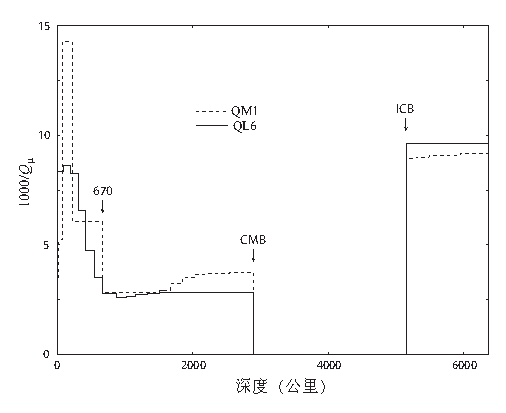
\includegraphics{../figures/chap09/fig17.eps}
\end{center}
\caption[Qmodels]{\label{9.fig.Qmods}
\index{Q@{\em Q} profile}%
\index{quality factor profile}%
$1000\hspace{0.4 mm}Q_{\mu}^{-1}$~随深度的变化:({\em 虚线\/})~QM1~模型~(Widmer, Masters \& Gilbert
\citeyear{widmer&al91});({\em 实线\/})~QL6~模型~(Durek \& Ekstr\"{o}m \citeyear{durek&ekstrom96})。图中标明了内核边界~(ICB)、核幔边界~(CMB)~和~670~km~间断面的位置。
}
\end{figure}
在所有晶体材料中,由位错运动和晶粒边界滑移等微观机制而引起的剪切衰减比体变衰减要大得多,因此在地球内部处处均有~$Q_{\kappa}\gg Q_{\mu}$~(Minster \citeyear{minster80}; Karato \& Spetzler \citeyear{karato&spetzler90})。然而,需要有少量的体变衰减,来解释观测到的径向及其他~PKIKP-等价模式的衰减率。QMl~模型的上地幔中~$Q_{\kappa}=2920$,液态外核中~$Q_{\kappa}=12,000$;QL6~模型的体变衰减稍大~($Q_{\kappa}=943$),局限在上地幔。Durek \& Ekstr\"{o}m
(\citeyear{durek&ekstrom95})~用他们在玻利维亚地震后改进的径向模式~$Q$~值数据对地幔内体变衰减的分布加以改善;他们的最优模型在软流圈(深度80--220~km)中~$Q_{\kappa}=213$,在其它区域~$Q_{\kappa}=27,700$。少量的体变耗散是地幔多晶性质预料中的结果---由于相邻晶粒弹性模量的局部差异,在宏观各向同性应力作用下,这种聚合体晶体内部会产生微观剪切应力。Jeanloz \& O'Connell (\citeyear{heinz&al82})~阐明,对于典型的地幔矿物组合,这一机制会导致~$Q_{\kappa}/Q_{\mu}\approx 50\!-\!100$。任何更大的软流圈体耗散,如果能够证实,可能意味着有部分熔融。目前几乎没有对固态内核敏感模式的可靠的衰减数据,因而内核中的~$Q_{\kappa}$~和~$Q_{\mu}$~均尚未很好地确定。

对简正模式和体波衰减测量数据的仔细比较,可以看到一些隐约但可靠的在地震波频段内~$Q_{\mu}$~随频率的增加而略微下降的证据,
\index{Q@{\em Q}!frequency dependence}%
径向传播的~${\rm ScS}_{\rm SH}$~或~${\rm ScS}_{\rm SV}$~波的理论品质因子为
\eq
Q_{\rm ScS}=\frac{\displaystyle{\int_b^a
\beta^{-1}\,dr}}{\displaystyle{\int_b^a
\beta^{-1}Q_{\beta}^{-1}\,dr}}
\en
在~QM1~模型中其数值为~$Q_{\rm ScS}=236\pm 5$,在~QL6~模型中为~$Q_{\rm ScS}=233\pm 5$;这些约束良好的数值适用于一个假想的超低频~(4~mhz)~波。直接用中等频率~(40~mHz)~多次反射~ScS~波衰减测量得到的数值在~$Q_{\rm ScS}=170\pm 34$~(Sipkin \& Jordan \citeyear{sipkin&jordan80})~到~$Q_{\rm ScS}=207\pm 25$~(Revenaugh \& Jordan \citeyear{revenaugh&jordan91})~之间。这两个结果之间的差异及其较大的不确定性反映了当区域性差异较大且地区性覆盖不均匀时,很难确定一个可靠的全球平均值;然而,从表面上看,这些结果意味着地幔的剪切衰减对十倍的频率增加有~10--20\%~的减小。对周期更短的~ScS~震相的常规性检测说明~$Q_{\mu}$~在~1~Hz~附近一定会再次增加。\textcite{sipkin&jordan79}~表阐,这种高频增加与在~$\tau_{\rm m}\approx 0.5$~秒存在一个吸收带边界是相符的。

已经有一些工作尝试利用钱德勒震颤来研究在地震波频段以下~$Q_{\mu}$~的行为,
\index{Chandler wobble}%
因为钱德勒震颤是以~435~天为周期对地球的非弹性进行采样。这些研究通常假设如~(\ref{6.powerQ})--(\ref{6.AndMin})~中一样的幂律关系~$Q_{\mu}\sim\omega^{\alpha}$,
\index{power-law $Q$ model}%
因而只是对指数~$\alpha$--这一个参数做估计。第一个进行这种研究的是~Jeffreys (\citeyear{jeffreys58a};
\citeyear{jeffreys58b});他用测量的钱德勒震颤的衰减率结合远震~S~波形没有强烈频散的定性观察得出“接近~$\alpha=0.17$”的结论。其他研究人员试图利用钱德勒震颤的周期和衰减率结合更新的地震资料来完善这一估计。\textcite{anderson&minster79}~得出的结论是“数据可以解释~$\alpha$大约为~0.2~到~0.4”,而~\textcite{smith&dahlen81}~在经过冗长的分析后确定~$0.04\leq\alpha\leq 0.19$。另一方面,Dickman (\citeyear{dickman88}; \citeyear{dickman93})~则发现证据与不依赖频率的非弹性相符合,即~$\alpha\approx 0$。最后两个结论之间的差异是由于难以计算明显不处于流体静力学平衡状态的弹性地球模型的钱德勒震颤的理论周期。重力或大地测量观测的固体地球的潮汐
与相应的章动、以及日长的每月与双周变化,可以用来约束在地震波频带与钱德勒震颤之间的四个数量级的频率差距上~$Q_{\mu}$~的行为。在过去,由于无法处理缺乏认识的大气和海洋效应,潮汐非弹性的研究受到阻碍~(Zschau \citeyear{zschau78}; \citeyear{zschau86};Wahr \& Bergen \citeyear{wahr&bergen86};Lambeck \citeyear{lambeck88})。然而,利用卫星雷达测高对开阔海洋潮汐的直接测量,已使这种情况在最近有所改善~(Ray, Eanes \& Chao \citeyear{ray&al96};Baker, Curtis \& Dodson \citeyear{baker&al96})。
\index{kernel!{\em Q}|)}%
\index{Q@{\em Q} kernel|)}%
\index{anelasticity|)}%
\index{attenuation|)}%
\index{Fr\'{e}chet kernel!anelastic|)}%

\renewcommand{\thesection}{$\!\!\!\raise1.3ex\hbox{$\star$}\!\!$
\arabic{chapter}.\arabic{section}}
%\section{Exact Anelasticity}
\section{精确非弹性}
\index{anelasticity!exact|(}%
\index{Rayleigh-Ritz method!SNRAI Earth|(}%
\renewcommand{\thesection}{\arabic{chapter}.\arabic{section}}

在上一节,我们应用瑞利原理推导了当~SNREI~地球模型的参数~$\kappa_0$、$\mu_0$、$\rho$~或横向各向同性地球模型的参数~$C_0$、$A_0$、$L_0$、$N_0$、$F_0$、$\rho$~有各向同性非弹性微扰时,其本征频率~$\om$~所产生的复数微扰~$\delta\om_d
+i\gamma$
\eq \label{9.expert1}
\kappa_0\rightarrow\kappa_0[1+iQ_{\kappa}^{-1}
+\twoinvpi Q_{\kappa}^{-1}\ln
(\om\hspace{-0.2 mm}/\hspace{-0.2 mm}\om_0)],
\en
\eq \label{9.expert2}
\mu_0\rightarrow\mu_0[1+iQ_{\mu}^{-1}
+\twoinvpi Q_{\mu}^{-1}\ln(\om\hspace{-0.2 mm}
/\hspace{-0.2 mm}\om_0)].
\en
(\ref{9.anel6})--(\ref{9.delwdisp})~这些常用的结果仅对非弹性的一阶成立;同时,径向本征函数~$U$、$V$~和~$W$~的相应微扰是被忽略的。事实上,只要稍微加一点努力,球对称非弹性地球模型的复数本征频率及其相应的本征函数基本上都可以精确地计算。一个直接的方法是在求解满足的一阶常微分方程和相应的边界条件时直接用~(\ref{9.expert1})--(\ref{9.expert2})~来分别替换~$\kappa$~和~$\mu$。\textcite{yuen&peltier82}~将这一方法用于均匀非弹性固体地球复数本征频率的解析计算,随后,Buland, Yuen, Konstanty \& Widmer~(\citeyear{buland&al85})~又用它在一个更真实的径向分层地球模型中以数值方法分析了非弹性对环型模式的影响。用数值方法找到如~(\ref{eq:8.det})~或~(\ref{eq:8.detfl})~那样的行列式方程的所有的复数根是非常困难的;由于这个原因,这种直接方法从未被应用于球型模式。另一种方法是用第~7~章讨论的~Rayleigh--Ritz~算法,经过一个简单的改变,来考虑弹性地球模型的振荡之间的非弹性耦合。我们在这里依照~\textcite{tromp&dahlen90b}~的描述,对这一数值上可行的方法做一个简要介绍。

有非弹性微扰的地球模型的球型和环型本征函数可以写为
\eq \label{9.exact1}
\bs^{\rm S}=\sU\bP_{lm}+\sV\bB_{lm},\qquad\bs^{\rm T}=\sW\bC_{lm},
\en
其中~$\bP_{lm}$、$\bB_{lm}$~和~$\bC_{lm}$~是~(\ref{8.PBClm})~中定义的实数矢量球谐函数。基本思路是将复数径向本征函数~$\sU$、$\sV$~和~$\sW$ ~用微扰前模型的实数本征函数~$U$、$V$~和~$W$~展开成~(\ref{7.RRexp})~式的形式:
\eq \label{9.RRexp}
\sU=\sum_nq_n^{\rm S}U_n,\qquad\sV=\sum_nq_n^{\rm S}V_n,
\qquad\sW=\sum_nq_n^{\rm T}W_n,
\en
这里我们要确定的是复数系数~$q_n^{\rm S}$~和~$q_n^{\rm T}$。由于~(\ref{9.expert1})--(\ref{9.expert2})~所给定的微扰的球对称性,不存在球型--环型耦合,也不存在类型相同但角次数~$l$~或级数~$m$~不同的模式之间的耦合。仅有的耦合是类型与次数~$l$~均相同的环型模式~${}_n{\rm T}_l\!-\!{}_{n'}{\rm T}_l$~之间或球型模式~${}_n{\rm S}_l\!-\!{}_{n'}{\rm S}_l$~之间的耦合。因此,(\ref{9.RRexp})~中的求和角标仅为径向阶数~$n$。为简单起见,我们采用简化符号,分别用~$U_n$、$V_n$~和~$W_n$~表示~${}_nU_l$、${}_nV_l$~和~${}_nW_l$,类似地,将微扰前本征频率~${}_n\om_l$~用~$\om_n$~表示。

将表达式~(\ref{9.exact1})--(\ref{9.RRexp})~代入线性化运动方程~(\ref{eq:8.eqmot}),用任一弹性本征函数~$U_n\bP_{lm}+V_n\bB_{lm}$~或~$W_n\bC_{lm}$~点乘所得结果,在地球模型~$\earth$~内部做部分积分。并利用边界条件~(\ref{eq:8.df})--(\ref{eq:8.dfs})。由此得到一对如下形式的非线性~$\infty\times\infty$~代数本征值方程
\eq
[\ssOmega^2+i\ssA+\twoinvpi
\ln(\om\hspace{-0.2 mm}/\hspace{-0.2 mm}
\om_0)\hspace{0.2 mm}\ssA]\hspace{0.2 mm}\ssq=(\om
+i\gamma)^2\ssq,
\label{eq:9.mateq}
\en
其中~$\ssq$~为未知的展开系数~$q_n^{\rm S}$~或~$q_n^{\rm T}$~组成的列向量,$\ssOmega$~为微扰前本征频率~$\om_n^{\rm S}$~或~$\om_n^{\rm T}$~组成的对角矩阵,$\ssA$~为非弹性势能微扰矩阵,其分量表达式为
\eqa \label{9.matel}
\lefteqn{A_{nn'}^{\rm S}=\int_0^a
\Big\{\kappa_0Q_{\kappa}^{-1}
(r\dU_{\!n}+2U_n-\sqL V_n)
(r\dU_{\!n'}+2U_{n'}-\sqL V_{n'})} \nonumber \\
&&\mbox{}+\mu_0Q_{\mu}^{-1}\big[\third(2r\dU_{\!n}-2U_n+\sqL V_n)
(2r\dU_{\!n'}-2U_{n'}+\sqL V_{n'})
\nonumber \\
&&\mbox{}\qquad+(r\dV_{\!n}-V_n+\sqL U_n)
(r\dV_{\!n'}-V_{n'}+\sqL U_{n'}) \nonumber \\
&&\mbox{}\qquad\quad+(\sqL^2-2)V_nV_{n'}\big]
\Big\}\,dr,
\ena
\eqa \label{9.matel2}
\lefteqn{A_{nn'}^{\rm T}=\int_0^a
\mu_0Q_{\mu}^{-1}
\big[(r\dW_{\!n}-W_n)(r\dW_{\!n'}-W_{n'})} \nonumber \\
&&\mbox{}\qquad\quad\hspace{4.0 mm}
+(\sqL^2-2)W_nW_{n'}\big]\,dr.
\ena
通过迭代求解方程~(\ref{eq:9.mateq})~的截断形式,可以得到球对称非弹性地球的复数本征频率~$\om
+i\gamma$~及其相应的径向本征函数~$\sU$、$\sV$~和~$\sW$。矩阵~$\ssA$~的维度恰好是分析中所考虑的径向阶数目,因而该方法在计算上较为简单。

对称性~$A_{n'n}^{\rm S}=A_{nn'}^{\rm S}$~和~$A_{n'n}^{\rm T}=A_{nn'}^{\rm T}$~确保复数球型和环型本征函数在下述意义上是双正交的
\index{biorthogonality!SNRAI Earth}%
\index{biorthonormality!SNRAI Earth}%
\eqa \label{9.biortho}
\lefteqn{\int_b^a\rho\hspace{0.2 mm}(\sU_n\sU_{n'}+\sV_n\sV_{n'})\,r^2dr
-\frac{2}{\pi}\frac{\ln(\om_n/\om_{n'})}
{\om_n^2-\om_{n'}^2}} \nonumber \\
&&\mbox{}\times\int_0^a\Big\{\kappa_0Q_{\kappa}^{-1}
(r\hspace{0.2 mm}\dot{\sU}_n+2\hspace{0.4 mm}\sU_n-\sqL\sV_n)
(r\hspace{0.2 mm}\dot{\sU}_{n'}+2\hspace{0.4 mm}
\sU_{n'}-\sqL\sV_{n'}) \nonumber \\
&&\mbox{}\quad+\mu_0Q_{\mu}^{-1}
\big[\third(2r\hspace{0.2 mm}\dot{\sU}_n-2\hspace{0.4 mm}\sU_n+\sqL\sV_n)
(2r\hspace{0.2 mm}\dot{\sU}_{n'}-2\hspace{0.4 mm}\sU_{n'}+\sqL\sV_{n'})
\nonumber \\
&&\mbox{}\quad\quad+(r\dot{\sV}_n-\sV_n+\sqL\hspace{0.4 mm}\sU_n)
(r\dot{\sV}_{n'}-\sV_{n'}+\sqL\hspace{0.4 mm}\sU_{n'}) \nonumber \\
&&\mbox{}\quad\quad\quad+(\sqL^2-2)\sV_n\sV_{n'}\big]
\Big\}\,dr=0\quad\mbox{if
$\om_n\neq\om_{n'}$,}
\ena
\eqa
\lefteqn{\int_0^a\rho\hspace{0.2 mm}\sW_n\sW_{n'}\,r^2dr
-\frac{2}{\pi}\frac{\ln(\om_n/\om_{n'})}
{\om_n^2-\om_{n'}^2}} \nonumber \\
&&\mbox{}\times\int_0^a\mu_0Q_{\mu}^{-1}
\big[(r\dot{\sW}_n-\sW_n)(r\dot{\sW}_{n'}-\sW_{n'}) \nonumber \\
&&\mbox{}\quad\quad\quad+(\sqL^2-2)\sW_n\sW_{n'}\big]\,dr=0\quad\mbox{if
$\om_n\neq\om_{n'}$.}
\ena
在~$\om_{n'}\rightarrow\om_n$~极限情形下,相应的归一化条件为
\eqa
\lefteqn{\int_0^a\rho\hspace{0.2 mm}(\sU_n^2+\sV_n^2)\,r^2dr
-\frac{1}{\pi}\om_n^{-2}\int_0^a\Big\{\kappa_0Q_{\kappa}^{-1}
(r\hspace{0.2 mm}\dot{\sU}_n+2\hspace{0.4 mm}\sU_n-\sqL\sV_n)^2}
\nonumber \\
&&\mbox{}+\mu_0Q_{\mu}^{-1}
\big[\third(2r\hspace{0.2 mm}\dot{\sU}_n-2\hspace{0.4 mm}
\sU_n+\sqL\sV_n)^2
+(r\dot{\sV}_n-\sV_n+\sqL\hspace{0.4 mm}\sU_n)^2 \nonumber \\
&&\mbox{}\quad\quad\quad+(\sqL^2-2)\sV_n^2\big]
\Big\}\,dr=1,
\ena
\eqa \label{9.binorm2}
\lefteqn{\int_0^a\rho\hspace{0.2 mm}\sW_n^2\,r^2dr
-\frac{1}{\pi}\om_n^{-2}\int_0^a\mu_0Q_{\mu}^{-1}
\big[(r\dot{\sW}_n-\sW_n)^2} \nonumber \\
&&\mbox{}\quad\quad\quad+(\sqL^2-2)\sW_n^2\big]\,dr=1.
\ena
与微扰前本征函数一样,我们将~${}_n\sU_l$、${}_n\sV_l$~和~${}_n\sW_l$~简写为~$\sU_n$、$\sV_n$~和~$\sW_n$。(\ref{9.biortho})--(\ref{9.binorm2})~是无自转非弹性地球普遍双正交关系~(\ref{6.orthog})--(\ref{6.normal})~的一个特例。

\textcite{tromp&dahlen90b}~证明,通过求解本征值问题~(\ref{eq:9.mateq})~得到的衰减率~$\gamma=\half\om Q^{-1}$~普遍可以用由瑞利原理得到的~$Q^{-1}$~的一阶公式很好地近似。这证明在简正模式衰减的反演研究中继续使用近似式~(\ref{9.anel7})~是合理的。由于微扰前本征频率之间的规则间距,球对称非弹性耦合对环型模式~${}_n{\rm T}_l$~的影响可以忽略不计。受它们影响最强的是微扰前具有几乎简并本征频率的球型模式~${}_n{\rm S}_l$,这些模式位于沿~PKIKP-等价、${\rm ScS}_{\rm SV}$-等价和~${\rm J}_{\rm SV}$-等价频散分支上规避的交叉点附近。对于少数强耦合模式,通过求解方程~(\ref{eq:9.mateq})~得到的频散本征频率偏移~$\om-\om_n$~与由~(\ref{9.delwdisp})~给定的相应的一阶偏移可能相差一到两个~$\mu\mbox{Hz}$,这与许多本征频率测量的精度量级相同。此外,一些强耦合模式的复数本征函数~$\sU_n$~和~$\sV_n$~与相应的微扰前实数本征函数~$U_n$~和~$V_n$~可能有巨大差异。这会对地震后相应振荡的理论相位和幅度有重大影响。所幸的是,异常最大的模式主要是~${\rm J}_{\rm SV}$~等价的内核模式,这些模式既难以激发又难以观测。

\begin{table}[tb]
\centering
\begin{tabular}{|c|c|} \hline
& \\
$\displaystyle{{\raisebox{-0.2ex}{\rm 球对称}}
\atop{\raisebox{0.2ex}{\rm 地球模型}}}$
& $\displaystyle{{\raisebox{-0.2ex}{\rm 精确的或零阶}}
\atop{\raisebox{0.2ex}{\rm 位移本征函数}}}$ \\
& \\ \hline
& \\
$\displaystyle{{\raisebox{-1.0ex}{\rm 无自转}}\atop{\raisebox{1.0ex}{\rm 弹性}}}$
& $\displaystyle{\bs=U\brh\sY_{lm}+k^{-1}V\,\bdel_{\!1}\sY_{lm}
-k^{-1}W(\brh\times\bdel_{\!1}\sY_{lm})}$ \\
& \\
$\displaystyle{{\raisebox{-1.0ex}{\rm 自转}}\atop{\raisebox{1.0ex}{\rm 弹性}}}$
& $\displaystyle{\bs=U\brh Y_{lm}+k^{-1}V\,\bdel_{\!1}Y_{lm}
-k^{-1}W(\brh\times\bdel_{\!1}Y_{lm})}$ \\
& \\
$\displaystyle{{\raisebox{-1.0ex}{\rm 无自转}}\atop{\raisebox{1.0ex}{\rm 非弹性}}}$
& $\displaystyle{\bs=\sU\brh\sY_{lm}+k^{-1}\sV\,\bdel_{\!1}\sY_{lm}
-k^{-1}\sW(\brh\times\bdel_{\!1}\sY_{lm})}$ \\
& \\
$\displaystyle{{\raisebox{-1.0ex}{\rm 自转}}\atop{\raisebox{1.0ex}{\rm 非弹性}}}$
& $\displaystyle{\bs=\sU\brh Y_{lm}+k^{-1}\sV\,\bdel_{\!1}Y_{lm}
-k^{-1}\sW(\brh\times\bdel_{\!1}Y_{lm})}$ \\
& \\ \hline
\end{tabular}
\caption[Four eigenfunctions]{
有无自转和非弹性的球对称地球模型的位移本征函数。标量函数~$U$、$V$、$W$~和球谐~$\sY_{lm}$~均为实数,而~$\sU$、$\sV$、$\sW$~和~$Y_{lm}$~则均为复数。环型本征函数有~$U=V=0$~和~$\sU=\sV=0$,而球型本征函数有~$W=0$~和~$\sW=0$。无自转球对称地球模型的本征函数是精确的,而自转球对称地球模型的本征函数则仅精确到自转角速率~$\Omega=\|\mbox{\boldmath $\Omega$}\|$~的零阶。
}
\end{table}

在本章的结尾,我们提醒大家留意在表达式~(\ref{9.exact1})~中使用实数矢量球谐函数~$\bP_{lm}=\brh\sY_{lm}$、$\bB_{lm}=k^{-1}\bdel_{\!1}\sY_{lm}$~和~$\bC_{lm}=-k^{-1}(\brh\times\bdel_{\!1}\sY_{lm})$~的必要性。
\index{spherical harmonics!real}%
\index{real spherical harmonics}%
如果我们试图用复数矢量谐函数~$\brh Y_{lm}$、$k^{-1}\bdel_{\!1}Y_{lm}$~和~$-k^{-1}(\brh\times\bdel_{\!1}Y_{lm})$~来表示~$\bs^{\rm S}$~和~$\bs^{\rm T}$,那么矢量双正交关系~(\ref{6.orthog})--(\ref{6.normal})~式就~{\em 不会\/}简化为标量关系~(\ref{9.biortho})--(\ref{9.binorm2})。非弹性本征函数~$\bs^{\rm S}$~和~$\bs^{\rm T}$~所仅有的复杂性一定是在径向标量函数~$\sU$、$\sV$~和~$\sW$~中所固有的;在第~\ref{10.sec.Green}~节中我们会看到,这是在无自转、球对称非弹性地球上简正模式激发的计算中必不可少的。地球的自转在地区上和径向上都带来复杂性;事实上,精确到~$\Omega=\|\bOmega\|$~的零阶,自转的弹性或非弹性地球的本征函数与对应的无自转地球的本征函数完全一样,只要把~$\sY_{lm}$~
用~$Y_{lm}$~替换~(见第~14.2.1~节)。在表~9.1~中,我们归纳了在是否考虑自转和非弹性时精确的或零阶本征函数的特质。
\index{anelasticity!exact|)}%
\index{Rayleigh-Ritz method!SNRAI Earth|)}%